%% For double-blind review submission, w/o CCS and ACM Reference (max submission space)
%\documentclass[sigplan,review,anonymous]{acmart}\settopmatter{printfolios=true,printccs=false,printacmref=false}
%% For double-blind review submission, w/ CCS and ACM Reference
%\documentclass[acmsmall,review,anonymous]{acmart}\settopmatter{printfolios=true}
%% For single-blind review submission, w/o CCS and ACM Reference (max submission space)
%\documentclass[acmsmall,review]{acmart}\settopmatter{printfolios=true,printccs=false,printachttps://www.overleaf.com/project/5eb13412d04a610001998594mref=false}
%% For single-blind review submission, w/ CCS and ACM Reference
%\documentclass[acmsmall,review]{acmart}\settopmatter{printfolios=true}
%% For final camera-ready submission, w/ required CCS and ACM Reference
\documentclass[sigplan,screen]{acmart}\settopmatter{}


%% Journal information
%% Supplied to authors by publisher for camera-ready submission;
%% use defaults for review submission.
%\acmJournal{PACMPL}
%\acmVolume{1}
%\acmNumber{ICFP} % CONF = POPL or ICFP or OOPSLA
%\acmArticle{1}
%\acmYear{2020}
%\acmMonth{5}
%\acmDOI{} % \acmDOI{10.1145/nnnnnnn.nnnnnnn}
%\acmConference[Haskell'20]{13th ACM SIGPLAN International Haskell Symposium}{August 27-28, 2020}{New Jersey, United States}

%%% If you see 'ACMUNKNOWN' in the 'setcopyright' statement below,
%%% please first submit your publishing-rights agreement with ACM (follow link on submission page).
%%% Then please update our instructions page and copy-and-paste the NEW commands into your article.
%%% Please contact us in case of questions; allow up to 10 min for the system to propagate the information.
%%%
%%% The following is specific to Haskell '20 and the paper
%%% 'Type Your Matrices for Great Good: A Haskell Library of Typed Matrices and Applications (Functional Pearl)'
%%% by Armando Santos and José N. Oliveira.
%%%
\setcopyright{acmcopyright}
\acmPrice{15.00}
\acmDOI{10.1145/3406088.3409019}
\acmYear{2020}
\copyrightyear{2020}
\acmSubmissionID{icfpws20haskellmain-p16-p}
\acmISBN{978-1-4503-8050-8/20/08}
\acmConference[Haskell '20]{Proceedings of the 13th ACM SIGPLAN International Haskell Symposium}{August 27, 2020}{Virtual Event, USA}
\acmBooktitle{Proceedings of the 13th ACM SIGPLAN International Haskell Symposium (Haskell '20), August 27, 2020, Virtual Event, USA}

\startPage{1}

%% Copyright information
%% Supplied to authors (based on authors' rights management selection;
%% see authors.acm.org) by publisher for camera-ready submission;
%% use 'none' for review submission.
%\setcopyright{none}
%\setcopyright{acmcopyright}
%\setcopyright{acmlicensed}
%\setcopyright{rightsretained}
%\copyrightyear{2018}           %% If different from \acmYear

%% Bibliography style
\bibliographystyle{ACM-Reference-Format}
%% Citation style
%% Note: author/year citations are required for papers published as an
%% issue of PACMPL.
\citestyle{acmauthoryear}   %% For author/year citations

%%%%%%%%%%%%%%%%%%%%%%%%%%%%%%%%%%%%%%%%%%%%%%%%%%%%%%%%%%%%%%%%%%%%%%
%% Note: Authors migrating a paper from PACMPL format to traditional
%% SIGPLAN proceedings format must update the '\documentclass' and
%% topmatter commands above; see 'acmart-sigplanproc-template.tex'.
%%%%%%%%%%%%%%%%%%%%%%%%%%%%%%%%%%%%%%%%%%%%%%%%%%%%%%%%%%%%%%%%%%%%%%

%% Some recommended packages.
\usepackage{booktabs}   %% For formal tables:
                        %% http://ctan.org/pkg/booktabs
\usepackage{subcaption} %% For complex figures with subfigures/subcaptions
                        %% http://ctan.org/pkg/subcaption
                        
\usepackage{caption}
\newenvironment{code}{\captionsetup{type=listing}}{}

\usepackage{multicol}

\usepackage{tikz-cd}
\usepackage{mathtools}
\usepackage{minted}
\setminted[haskell]{escapeinside=\\@\\@, fontsize=\small}
\newcommand{\hs}{\mintinline{haskell}}
\usepackage{xcolor}
\definecolor{wine}{RGB}{139, 63, 69}
\def\wine{\color{wine}}

%----- jno added stuff -----
%\usepackage{fleqn}
%\setlength\mathindent{3em}
\usepackage{multirow}
\newenvironment{lcbr}{\left\{\begin{array}{l}}{\end{array}\right.}
\usepackage[all]{xy}
\def\rarrow#1#2#3{\def\nolabel{}\def\lab{#2}\ifx\lab\nolabel{#1\to #3}\else\xymatrix{ #1 \ar[r]^-{#2} & #3 }\fi}
\def\larrow#1#2#3{\def\nolabel{}\def\lab{#2}\ifx\lab\nolabel{#3\from#1}\else\xymatrix{ #3 & #1 \ar[l]_-{#2}}\fi}
\def\longlarrow#1#2#3{\xymatrix{ #3 && #1 \ar[ll]_-{#2} }}
\def\longrarrow#1#2#3{\xymatrix{ #1 \ar[rr]^-{#2} && #3 }}
\usepackage{wrapfig}
\def\doc{paper}
\def\start{&&}
\def\more{\\&&}
\def\just#1#2{\\ &#1& \rule{2em}{0pt} \{ \mbox{\rule[-.7em]{0pt}{1.8em} \small #2 \/} \} \nonumber\\ && }
\def\conv#1{#1^\circ}
\def\comp{ \mathbin{\cdot} }
\def\kr{\mathbin{\hbox{\tiny${}^\triangledown$}}}
\let\kons=\underline
\def\xsor{{\dot\vee}}
%--------------------------
\def\msplit#1#2{\left[\begin{array}{c}#1\\\hline#2\end{array}\right]} % Split
\def\meither#1#2{\left[\begin{array}{c|c}{#1}&{#2}\end{array}\right]} % either
\def\matfour#1#2#3#4{\begin{bmatrix} \left.\begin{matrix} \dfrac{#1}{#3} \end{matrix}\ \right|\ \begin{matrix} \dfrac{#2}{#4} \end{matrix}\end{bmatrix}}
%---------------------------
\def\cnot{
\begin{picture}(70.00,60.00)(0,-5)
\put(10.00,16.00){\dashbox{2.00}(40.00,47.00)[cc]{}}
\put(60.00,45.00){\makebox(20.00,16.00)[cc]{$a'$}}
\put(60.00,25.00){\makebox(20.00,16.00)[cc]{$b'$}}
\put(-15.00,44.00){\makebox(20.00,16.00)[cc]{$a$}}
\put(-15.00,24.00){\makebox(20.00,16.00)[cc]{$b$}}
\put(0.00,52.00){\line(1,0){60.00}}
\put(0.00,32.00){\line(1,0){60.00}}
\put(30.00,52.00){\circle*{5.00}}
\put(30.00,32.00){\circle{10.00}}
\put(30.00,52.00){\line(0,-1){25.00}}
\end{picture}}
\def\toffoli{
\begin{picture}(70.00,80.00)(10,10)
\put(10.00,20.00){\dashbox{2.00}(40.00,60.00)[cc]{}}
\put(-15.00,58.00){\makebox(20.00,16.00)[cc]{$a$}}
\put(60.00,59.00){\makebox(20.00,16.00)[cc]{$a'$}}
\put(60.00,45.00){\makebox(20.00,16.00)[cc]{$b'$}}
\put(60.00,25.00){\makebox(20.00,16.00)[cc]{$c'$}}
\put(-15.00,44.00){\makebox(20.00,16.00)[cc]{$b$}}
\put(-15.00,24.00){\makebox(20.00,16.00)[cc]{$c$}}
\put(0.00,67.00){\line(1,0){60.00}}
\put(0.00,52.00){\line(1,0){60.00}}
\put(0.00,32.00){\line(1,0){60.00}}
\put(30.00,67.00){\circle*{5.00}}
\put(30.00,52.00){\circle*{5.00}}
\put(30.00,32.00){\circle{10.00}}
\put(30.00,67.00){\line(0,-1){40.00}}
\end{picture}} 
%---------------------------
\usepackage{circuitikz}
\def\toffolicore{%
\begin{circuitikz}
\draw
(0,1) node (and) [xshift=1cm,and port, scale=.8]   {}
(3,0.5) node (xor) [xor port, scale=.8]            {}
(and.in 1) node (A1)     [anchor=east,xshift=-1cm]  {$a$}
(and.in 2) node (B1)     [anchor=east,xshift=-1cm]  {$b$}
(xor.in 2) node (C1)     [anchor=east,xshift=-3cm]  {$c$}
(xor.out) node (Z1)      [anchor=east,xshift= 1.6cm]  {$z$};
\draw
        (and.out) |- (xor.in 1)
        (and.in 1) -- (A1)
        (and.in 2) -- (B1)
        (xor.in 2) -- (C1)
        (xor.out) -- (Z1);
\end{circuitikz}}
%---------------------------

%---- Camera-ready stuff -----
\usepackage{microtype}

\begin{document}

%% Title information
\title{ %Typed Matrices à la LAoP
          %Type Polymorphism in Linear Algebra 
          Type Your Matrices for Great Good}         %% [Short Title] is optional;
                                        %% when present, will be used in
                                        %% header instead of Full Title.
%\titlenote{LAoP - Linear Algebra of Programming}             %% \titlenote is optional;
                                        %% can be repeated if necessary;
                                        %% contents suppressed with 'anonymous'
\subtitle{A Haskell Library of Typed Matrices and Applications (Functional Pearl)}                     %% \subtitle is optional
%\subtitlenote{with subtitle note}       %% \subtitlenote is optional;
                                        %% can be repeated if necessary;
                                        %% contents suppressed with 'anonymous'


%% Author information
%% Contents and number of authors suppressed with 'anonymous'.
%% Each author should be introduced by \author, followed by
%% \authornote (optional), \orcid (optional), \affiliation, and
%% \email.
%% An author may have multiple affiliations and/or emails; repeat the
%% appropriate command.
%% Many elements are not rendered, but should be provided for metadata
%% extraction tools.

%% Author with single affiliation.
\author{Armando Santos}
%\authornote{with author1 note}          %% \authornote is optional;
                                        %% can be repeated if necessary
%\orcid{nnnn-nnnn-nnnn-nnnn}             %% \orcid is optional
\affiliation{
  \position{}
  \department{High Assurance Software Laboratory}              %% \department is recommended
  \institution{INESC TEC and University of Minho}            %% \institution is required
  \streetaddress{}
  \city{Braga}
  \state{Portugal}
  \postcode{}
  \country{Portugal}                    %% \country is recommended
}
\email{armando.j.santos@inesctec.pt}          %% \email is recommended

%% Author with single affiliation.
\author{José N. Oliveira}
%\authornote{with author1 note}          %% \authornote is optional;
                                        %% can be repeated if necessary
%\orcid{nnnn-nnnn-nnnn-nnnn}             %% \orcid is optional
\affiliation{
  \position{}
  \department{High Assurance Software Laboratory}              %% \department is recommended
  \institution{INESC TEC and University of Minho}            %% \institution is required
  \streetaddress{}
  \city{Braga}
  \state{Portugal}
  \postcode{}
  \country{Portugal}                    %% \country is recommended
}
\email{jno@di.uminho.pt}          %% \email is recommended

%% Author with two affiliations and emails.
%\author{First2 Last2}
%\authornote{with author2 note}          %% \authornote is optional;
%                                        %% can be repeated if necessary
%\orcid{nnnn-nnnn-nnnn-nnnn}             %% \orcid is optional
%\affiliation{
%  \position{Position2a}
%  \department{Department2a}             %% \department is recommended
%  \institution{Institution2a}           %% \institution is required
%  \streetaddress{Street2a Address2a}
%  \city{City2a}
%  \state{State2a}
%  \postcode{Post-Code2a}
%  \country{Country2a}                   %% \country is recommended
%}
%\email{first2.last2@inst2a.com}         %% \email is recommended
%\affiliation{
%  \position{Position2b}
%  \department{Department2b}             %% \department is recommended
%  \institution{Institution2b}           %% \institution is required
%  \streetaddress{Street3b Address2b}
%  \city{City2b}
%  \state{State2b}
%  \postcode{Post-Code2b}
%  \country{Country2b}                   %% \country is recommended
%}
%\email{first2.last2@inst2b.org}         %% \email is recommended


%% Abstract
%% Note: \begin{abstract}...\end{abstract} environment must come
%% before \maketitle command
\begin{abstract}
We study a simple inductive data type for representing correct-by-construction matrices. Despite its simplicity, it can be used to implement matrix-manipulation algorithms efficiently and safely, performing in some cases faster than existing alternatives even though the algorithms are written in a direct and purely functional style. A rich collection of laws makes it possible to derive and optimise these algorithms using equational reasoning, avoiding the notorious off-by-one indexing errors when fiddling with matrix dimensions. We demonstrate the usefulness of the data type on several examples, and highlight connections to related topics in category theory.
\end{abstract}

%% 2012 ACM Computing Classification System (CSS) concepts
%% Generate at 'http://dl.acm.org/ccs/ccs.cfm'.
\begin{CCSXML}
<ccs2012>
<concept>
<concept_id>10002950</concept_id>
<concept_desc>Mathematics of computing</concept_desc>
<concept_significance>500</concept_significance>
</concept>
</ccs2012>
\end{CCSXML}

\ccsdesc[500]{Mathematics of computing}
%% End of generated code

%% Keywords
%% comma separated list
\keywords{Haskell, Linear Algebra of Programming, Matrices, Probabilistic Programming, Quantum Programming, Data Analysis}  %% \keywords are mandatory in final camera-ready submission


%% \maketitle
%% Note: \maketitle command must come after title commands, author
%% commands, abstract environment, Computing Classification System
%% environment and commands, and keywords command.
\maketitle

\section{Introduction}\label{sec-intro}

Matrices are central to mathematics and computer science, from linear algebra and probability theory to machine learning and computer graphics. Matrices play an important role in problem specification as well as in finding efficient solutions, for which exists specialised hardware processing units~\cite{volkov2008benchmarking,sato2017depth}.

But what is a matrix really? A matrix is commonly viewed as an array of elements arranged in rows and columns. In textbooks, a matrix $A$ with $c$ columns and $r$ rows is typically pictured as a rectangular area whose elements $a_{ij}$ are numbers (or expressions denoting them):
\begin{equation*}
A =
  \begin{bmatrix}
    a_{11} & \ldots & a_{1c}\\
    \vdots & \ddots & \vdots \\
    a_{r1} & \ldots & a_{rc}
  \end{bmatrix}
\end{equation*}{}

It is not surprising that software developers often translate this array-based matrix representation directly into code when implementing matrix algorithms. For dense matrices, this can give excellent results in terms of performance, but programming against such a low-level representation is challenging and ill-suited for purely functional programming languages.

On the other hand, matrix manipulation very often operates over \emph{blocks} rather than over individual cell values, for instance over the three blocks of matrix \( A = \meither B {\frac C D}\). In such cases, awkward, error-prone index calculations could remain implicit if smart matrix-block combinators were used.

This paper views matrices as inductive structures that can be constructed from simple primitives, as captured by the following data type\footnote{This paper uses Haskell but the presented ideas can be adapted to other functional programming languages.}:

\vspace{1mm}
\begin{minted}[xleftmargin=10pt]{haskell}
data Matrix e c r where
  One   :: e -> Matrix e () ()
  Join  :: Matrix e a r -> Matrix e b r 
        -> Matrix e (Either a b) r
  Fork  :: Matrix e c a -> Matrix e c b 
        -> Matrix e c (Either a b)
\end{minted}
\vspace{1mm}

\noindent
Here the type variable \hs{e} stands for the type of the matrix \emph{elements}, while \hs{c} (\emph{columns}) and \hs{r} (\emph{rows}) specify the dimensions. This data type will be discussed in more detail in~\S\ref{sec-matrix-type}; for now, we would like to emphasise that matrix dimensions appear only at the type level, i.e.\ it is impossible to make any dimension or indexing errors while constructing a value of type \hs{Matrix}~\hs{e}~\hs{c}~\hs{r}.

This data type is matrix-block-oriented and particularly suitable to express block operations which, as will be seen soon, are very common and rely on a sound mathematical basis.

\subsection{Contributions}

This \doc\ presents a \emph{type safe inductive matrix data structure} definition, exposing its biproduct architecture and equipped with a matrix programming library in Haskell, that stands out from the rest for having an inductive definition that enables writing statically typed matrix manipulation functions in a more elegant, calculational and efficient way.

The main goal of this paper is to demonstrate that by taking advantage of a strongly typed functional programming language, one can write and reason about elegant and composable linear algebra programs. Our specific contributions are:

\begin{itemize}
    \item We develop a library for transforming and manipulating matrices and demonstrate its composability and flexibility.
    \item Compared to current libraries, ours is more compositional and polymorphic and does not have partial matrix manipulation functions (hence less chances for usage errors). 
    \item Our implementation of matrices enables simple manipulation of submatrices, making it particularly suitable for formal verification and equation reasoning, using the mathematical framework defined by the linear algebra of programming \citep{oliveira2012towards}. Furthermore, the data type constructors ensure that the matrices of this kind are sound, i.e. malformed matrices with incorrect dimensions of the sort, can not be constructed.
    \item Some practical examples that use the proposed matrix library in several application domains (e.g.\ probabilistic programming, quantum programming) are given and show how functional programming blends naturally with linear algebra. 
\end{itemize}{}

\subsection{Layout of the \doc}

%The motivation for the work developed is given in \S\ref{sec-motivation}.
The rest of the paper is structured as follows. A brief overview of the \textbf{Mat} category is given in \S\ref{sec-struct-mat} showing the rich algebra of matrices that emerges from the categorical notion of \emph{biproduct}.
% of programming discipline and obtain a new framework where proofs become simpler.
The core representation of the proposed inductive matrix type unfolds in \S\ref{sec-matrix-type}, followed by a concise explanation of how to write matrix manipulation functions around it (\S\ref{sec:200303a} to \S\ref{sec-manipulation}). Finally, some practical examples in the areas of probabilistic programming, quantum programming are given in \S\ref{sec-appl}, including evaluation. Related work, analysis of the proposed approach and directions for future research are discussed in sections \S\ref{sec-related-work} and \S\ref{sec-conclusion}, respectively.

\section{Background}\label{sec-motivation}

Category theory \cite{MA71, Awodey:2010:CT:2060081} is often referred to as a "theory of everything" because it is a framework where a lot of mathematical structures fit in. It has, in particular, a strong presence in functional programming \cite{Hi13, milewski2018category}. Such an abstract approach is relevant because abstraction plays a major role in computing \cite{Kr07}. 
%When designing an interface this should reveal as little as possible about the implementation details, making it possible to switch from the current implementation to an alternative one, i.e.\ to another \emph{instance} of the same \emph{concept}.
Category theory uses arrows as a generic notation able to cope with very distinct problem domains. These arrows, also called \emph{morphisms}, are typed with source and target objects and need to satisfy certain properties in order to form a category.

A standard way to achieve typed functional programming is to use the category \textbf{Set} of sets to type functions. For instance, in addition to the function definition:
\begin{align*}
    f x = x + 1
\end{align*}
\noindent an arrow between sets is added in order to constraint the scope of the function application:
\begin{align*}
    & f :: \mathbb{N} \longrightarrow \mathbb{N} \\
    & f x = x + 1
\end{align*}
\noindent This makes sure that $f$ can only be applied to arguments that are natural numbers. If by any chance this function is applied to a real number instead, this will be regarded as a wrong sentence and discarded by type checking.

The aphorism \emph{functions are special cases of relations} means that a function $f :: A \longrightarrow B$ can also be typed in the wider category of binary relations, the \textbf{Rel} category. In general, a morphism $R :: A \longrightarrow B$ in \textbf{Rel} is a relation $R \subseteq A \times B$, for instance:
\begin{align*}
    & R :: Object \longrightarrow Colour \\
    & o\ R\ c = c\ \text{is a colour of}\ o
\end{align*}
A function $f :: A \longrightarrow B$ is viewed as a relation wherever one writes the input/output relationship $b = f(a)$.

Both functions and relations have advanced type systems supported by the underlying categories. What about matrices? Matrices generalise relations into quantified ones, also termed \emph{labelled} or \emph{weighted} relations, leading into the category \textbf{Mat} of typed matrices.\footnote{See e.g.\ \cite{MO13c}. Strictly speaking, there is one such category \textbf{Mat}$_k$ per cell-type $k$, but ignoring this detail will not harm this summary of the overall theory.} A matrix $M$ with $c$ columns and $r$ rows can be regarded as a function $M(n, m)$ that tells the quantity occupying each cell $(n,m)$, for $1 \leq n \leq r$,  $1 \leq m \leq c$. From a categorical perspective, $M$ can be regarded as a morphism $c \xrightarrow{M} r$ indicating that matrix $M$ is of type $c \longrightarrow r$. In this setting, matrix-matrix multiplication can be expressed by arrow composition:
\begin{equation}\label{mm-cat-comp}
\begin{tikzcd}
r & c \arrow[l, "M"'] & p \arrow[l, "N"'] \arrow[ll, "M \cdot N", bend left]
\end{tikzcd}
\end{equation}
\noindent It has been shown that other interesting combinators arise from so-called \emph{biproducts} in the \textbf{Mat} category, which capture block-matrix operations in a natural way \cite{MO13c}. 

\subsection{Structure of \textbf{Mat}}\label{sec-struct-mat}
The structure of the \textbf{Mat} category is described below. \newline Figure \ref{fig:cheat_sheet} provides a reference guide containing the main algebraic laws.

\subsubsection{Basic structure}

For every dimension $d$ there is a matrix $d \longrightarrow d$ which is the unit of composition, i.e.\ the (square) \emph{identity} matrix of size $d$:
\begin{equation}\label{eq-id}
\begin{tikzcd}
m \arrow[d, "M"'] & m \arrow[l, "id_m"'] \arrow[d, "M"] \arrow[ld, "M"'] \\
n                 & n \arrow[l, "id_n"]                                 
\end{tikzcd}\hspace{2.5cm}
    id_n \cdot M = M = M \cdot id_m 
\end{equation}{}
Under composition (\ref{mm-cat-comp}) matrices form a category whose objects are matrix dimensions and whose morphism $n \xrightarrow{M} m$, $k \xrightarrow{N} n$, etc are the matrices themselves \cite{MA71,MO13c}.
%
%subsection{Vectors as arrows}
\emph{Vectors} are special cases of matrices in which one of the dimensions is $1$, for instance:
\begin{center}
 $v = \begin{bmatrix}
v_1 \\ 
\vdots\\
v_r 
\end{bmatrix}$ 
and $w = \begin{bmatrix}w_1 & \ldots & w_c \end{bmatrix}$
\end{center}
Column vector $v$ is of type $1 \longrightarrow r$ ($1$ column and $r$ rows) and row vector $w$ is of type $c \longrightarrow 1$ ($1$ row and $c$ columns). The convention is that lowercase letters denote vectors and uppercase letters denote matrices.

%\subsection{Matrix converse}
\textbf{Mat} is a ``dagger category" in the sense that every matrix $M$ can be transposed by
%Matrix \emph{transposition} (converse) is captured simply by changing the shape of a matrix dimensions,
swapping rows with columns. We denote the transposition (converse) of matrix $c \xrightarrow{M} r$ by $r \xrightarrow{M^\circ} c$. As expected, the idempotence law (\ref{eq:idempotence}) and the contravariance law (\ref{eq:091206b}) hold.
%\begin{align}
%& (M^\circ)^\circ = M \\
%& (M \cdot N)^\circ = N^\circ \cdot M^\circ
%\end{align}
 
\subsubsection{Bilinearity}
Given two matrices $c \xrightarrow{M, N} r$ of the same type, it makes sense to add them entry-wise to obtain the matrix $M+N$, where the symbol $+$ promotes the underlying cell-level additive operator to the matrix-level. Likewise, the additive unit cell value $0$ is lifted to the matrix $0$ fully filled with $0$s.

Matrix $0$ is the \emph{unit} element of matrix addition (\ref{eq:111008a}) and the \emph{zero} (absorbent) element of matrix composition (\ref{eq:zero}).
%The expected laws of matrix addition (\ref{eq:111008a},\ref{eq:zero}) hold.
The fact that composition is \emph{bilinear} relative to $+$, as given by laws (\ref{bilinearity-1},\ref{bilinearity-2}), is central to linear algebra as a whole.
%\begin{align}\label{bilinearity-1}
%& M \cdot (N + P) = M \cdot N + M \cdot C \\ \label{bilinearity-2}
%& (N + P) \cdot M = N \cdot M + P \cdot M
%\end{align}

In the same way that $M + N$ promotes the addition of matrix cells to the addition of the matrices themselves, the same promotion may take place with respect to the whole cell-level algebra. For example, cell value multiplication results in a matrix multiplication, denoted by $M \times N$
% or simply as $MN$
(for $M$ and $N$ of the same type), also known as the Hadamard product, which is commutative, associative and distributive over addition (i.e.\ bilinear).

\subsubsection{Products and co-products}\label{laop-laws}

From law (\ref{eq:091206c}) on-wards, Fig.~\ref{fig:cheat_sheet} presents the basic algebra of matrix-block combinators that will be used throughout the rest of the \doc. The concept of a \emph{biproduct} is central to their characterisation,
%  of \textbf{Mat}, which combines
combining categorical products and co-products into a single construction.

The diagram below shows how biproducts relate to products and co-products in the \textbf{Mat} category, compare with (\ref{join-def}) and (\ref{fork-def}) in Figure \ref{fig:cheat_sheet}.
\begin{figure}[H]%[07]{r}{16em}
        %\begin{center}
\vskip -0em
        \begin{tikzcd}
                                                            &  & d                                                                                           &  &                                                               \\
a \arrow[rr, "i_1"', bend left] \arrow[rru, "A", bend left] &  & a + b \arrow[u, "{[A\mathbin|B]}"'] \arrow[ll, "\pi_1", bend left] \arrow[rr, "\pi_2"', bend right] &  & b \arrow[ll, "i_2", bend right] \arrow[llu, "B"', bend right] \\
                                                            &  & c \arrow[u, "{\left[\frac{C}{D}\right]}"'] \arrow[llu, "C", bend left] \arrow[rru, "D"', bend right]   &  &                                                              
        \end{tikzcd}
        %\end{center}{}
\end{figure}
Expressions $\left[A \mathbin| B\right]$ and $\left[\frac{C}{D}\right]$ will be read
"A join B" and "C fork D", respectively. These operators purport the effect
of putting matrices side by side and on top of one another, respectively.
% expressed in terms of definitions (\ref{join-def}) and (\ref{fork-def}) rewrite to (\ref{inj-rfl}) and (\ref{prj-rfl}), respectively. Thus both injections and projections "decompose" the identity matrix.
Using such operators, projections $\pi_1$, $\pi_2$ and injections $i_1$, $i_2$ "decompose" the identity matrix through the so-called \emph{reflection} laws (\ref{inj-rfl},\ref{prj-rfl}).

The well-formedness of matrix block construction is therefore ensured by static type checking.
% This is a very important detail, and
To ensure correct typing, typed linear algebra practitioners are encouraged to draw the type diagrams associated to the expressions and equations in mind.

\begin{figure*}%[H]
\begin{minipage}{0.95\textwidth}\small
\hrulefill\setlength\columnsep{50pt}
\begin{multicols}{2}
    \noindent \textbf{Composition}
\begin{align}
            & M \comp (N \comp Q) = (M \comp N) \comp Q
\\
            & M \comp id = M = id \comp M
\end{align}{}
    \noindent \textbf{Converse (transposition)}
\begin{align}
& (M^\circ)^\circ = M \label{eq:idempotence}
\\
& (M \cdot N)^\circ = N^\circ \cdot M^\circ \label{eq:091206b}
\end{align}
    \noindent \textbf{Additivity}
\begin{align}
& M + (N + Q) = (M + N) + Q
\\
& M + 0 = M = 0 + M \label{eq:111008a}
\\
& M \cdot 0 = 0 = 0 \cdot M \label{eq:zero}
\end{align}{}
    \noindent \textbf{Bilinearity}
\begin{align}\label{bilinearity-1}
& M \cdot (N + P) = M \cdot N + M \cdot P \\ \label{bilinearity-2}
& (N + P) \cdot M = N \cdot M + P \cdot M
\end{align}
    \noindent \textbf{Universal properties}
\begin{align} \label{eq:091206c}
&	X = \meither{A}{B} \iff
	\begin{lcbr}
	X \comp i_1 = A
\\
	X \comp i_2 = B
	\end{lcbr}
\\
& X = \msplit C D \iff
	\begin{lcbr}
            \pi_1 \comp X = C
            \\
            \pi_2 \comp X = D
	\end{lcbr}
	\label{eq:091206d}
\end{align}{}
    \noindent \textbf{Reflection}
\begin{align}
            & \left[i_1 | i_2\right] = id \label{inj-rfl} \\
            & \left[\frac{\pi_1}{\pi_2}\right] = id \label{prj-rfl}
\end{align}{}
    \noindent \textbf{Join and Fork}
        \begin{align}\label{join-def}
            & \left[A | B\right] = A \cdot \pi_1 + B \cdot \pi_2 \\ \label{fork-def}
            & \left[\frac{C}{D}\right] = i_1 \cdot C + i_2 \cdot D 
        \end{align}{}
    \noindent \textbf{Fusion}
    \begin{align}\label{fusion-join}
        & P \cdot \left[A|B\right] = \left[P \cdot A | P \cdot B\right] \\ \label{fusion-fork}
        & \left[\frac{A}{B}\right] \cdot P = \left[\frac{A \cdot P}{B \cdot P}\right]
    \end{align}
    \noindent \textbf{Absorption}
    \begin{align}\label{eq:101221f}
        & \left[A \mathbin| B\right] \comp (C \oplus D) = \left[ A \comp C \mathbin| B \comp D \right] \\ \label{eq:1012212f}
        & \left[\frac{A}{B}\right] \comp (C \oplus D) = \left[\frac{A \comp C}{B \comp D}\right]
    \end{align}
    \noindent \textbf{Cancellation}
    \begin{align}\label{cancel-join}
        \left[ A \mathbin| B \right] \cdot i_1 = A\ ,\ \left[ A \mathbin| B \right] \cdot i_2 = B \\ \label{cancel-fork}
        \pi_1 \cdot \left[ \frac{A}{B} \right] = A\ ,\ \pi_2 \cdot \left[ \frac{A}{B} \right] = B
    \end{align}
    \noindent \textbf{Divide and conquer}
    \begin{equation}\label{eq-divide-and-conquer}
        \left[A \mathbin| B\right] \cdot \left[\frac{C}{D}\right] = A \cdot C + B \cdot D
    \end{equation}
    \noindent \textbf{Converse duality}
    \begin{equation}\label{converse-duality}
        \left[A \mathbin| B\right]^\circ = \left[\frac{A^\circ}{B^\circ}\right]
    \end{equation}
    \noindent \textbf{Exchange} ("abide") law
    \begin{equation}\label{abide-law}
        \left[\left[\frac{A}{C}\right] | \left[\frac{B}{D}\right]\right] = \left[\frac{\left[A | B\right]}{\left[C | D\right]}\right]
    \end{equation}
    \noindent \textbf{Blocked addition}
    \begin{align}
        & \left[ A \mathbin| B \right] + \left[C \mathbin| D \right] = \left[A + C \mathbin| B + D\right] \\
        & \left[ \frac{A}{B} \right] + \left[ \frac{C}{D} \right] = \left[ \frac{A + C}{B + D}\right]
    \end{align}
    \noindent \textbf{Structural equality}
    \begin{align}
        & \left[ A \mathbin| B \right] = \left[C \mathbin| D \right] \iff A = C \land B = D \\
        & \left[ \frac{A}{B} \right] = \left[ \frac{C}{D} \right] \iff A = C \land B = D 
    \end{align}
\end{multicols}
\hrulefill
\end{minipage}
    \caption{Summary of the laws of block-linear-algebra enabled by biproducts. (Valid only if over the same biproduct.)}
    \label{fig:cheat_sheet}
\end{figure*}

The laws of Figure \ref{fig:cheat_sheet} enable one to calculate standard linear algebra rules and algorithms. 
See as example the calculation alongside of the
\emph{divide-and-conquer} law of matrix multiplication (\ref{eq-divide-and-conquer}), also known as 
block-multiplication.

%---------
%\begin{align*}
%    & \left[A | B \right] \cdot \left[ \frac{C}{D} \right] \\
%&\llap= \qquad \{\ \text{Fork definition (\ref{fork-def}})\ \} \\
%    & \left[A | B \right] \cdot (i_1 \cdot C + i_2 \cdot D) \\
%&\llap= \qquad \{\ \text{Bilinearity (\ref{bilinearity-1})}\ \}  \\
%    & \left[A | B \right] \cdot i_1 \cdot C + \left[A | B \right] \cdot i_2 \cdot D \\
%&\llap= \qquad \{\ \text{Cancellation (\ref{cancel-join})}\ \} \\
%    & A \cdot C + B \cdot D
%\end{align*}{}
\begin{wrapfigure}[9]{r}{13em}\small
\centering\def\arraystretch{1.3}
\vskip -1em\(
\begin{array}{ll}
    & \left[A | B \right] \cdot \left[ \frac{C}{D} \right] \\
&\llap= \qquad \{\ \text{fork definition (\ref{fork-def}})\ \} \\
    & \left[A | B \right] \cdot (i_1 \cdot C + i_2 \cdot D) \\
&\llap= \qquad \{\ \text{bilinearity (\ref{bilinearity-1})}\ \}  \\
    & \left[A | B \right] \cdot i_1 \cdot C + \left[A | B \right] \cdot i_2 \cdot D \\
&\llap= \qquad \{\ \text{cancellation (\ref{cancel-join})}\ \} \\
    & A \cdot C + B \cdot D
\end{array}
\)
\end{wrapfigure}
Looking at matrices as lists of lists, or arrays, or graphs is a rather poor perspective on linear algebra. Somewhat more useful is to focus on how matrices are built or partitioned and on which formal rules are there for handling their internal structure, as seen above. Explicit, painful, low-level matrix manipulation is a source of dubious code, which is error-prone and difficult to analyse. Looking at it from a higher, abstract point of view that relies on a sound mathematical theory provides both simplicity and reliability benefits.

\section{Matrix data type}\label{sec-matrix-type}

Putting theory into practice, a safe and minimalist inductive matrix data type is encoded in Haskell. This data type takes into account certain conditions needed in order to accommodate the advantages that a good type system and the quantitative extension of the algebra of programming have to offer: be polymorphic, have statically typed dimensions, be type-inference friendly, be correct-by-construction and amenable to elegant and calculational manipulation.

As already mentioned, matrices are typed according to their dimensions and dealing with natural numbers at the type level is something that is possible in some of the most recent functional typed languages \cite{bove2009brief, brady2013idris}, including Haskell. Thus, a first approach to designing the inductive type could be:
\begin{minted}[xleftmargin=10pt]{haskell}
data Matrix e (c :: Nat) (r :: Nat) where
  One   :: e -> Matrix e 1 1
  Join  :: Matrix e a r -> Matrix e b r 
        -> Matrix e (a + b) r
  Fork  :: Matrix e c a -> Matrix e c b 
        -> Matrix e c (a + b)
\end{minted}
However, when dealing with type families that are responsible for calculating simple natural number arithmetics such as \hs{(+)}, the compiler has a very hard time inferring the correct types when writing algorithms via pattern-matching, for example, given that addition is not injective \cite{stolarek2015injective}. The approach followed in this paper is then based on the following GADT \cite{peyton2006simple}:

\begin{minted}[xleftmargin=10pt]{haskell}
data Matrix e c r where
  One   :: e -> Matrix e () ()
  Join  :: Matrix e a r -> Matrix e b r 
        -> Matrix e (Either a b) r
  Fork  :: Matrix e c a -> Matrix e c b 
        -> Matrix e c (Either a b)
\end{minted}

\begin{figure}%[9]{r}{18em}
\centering
  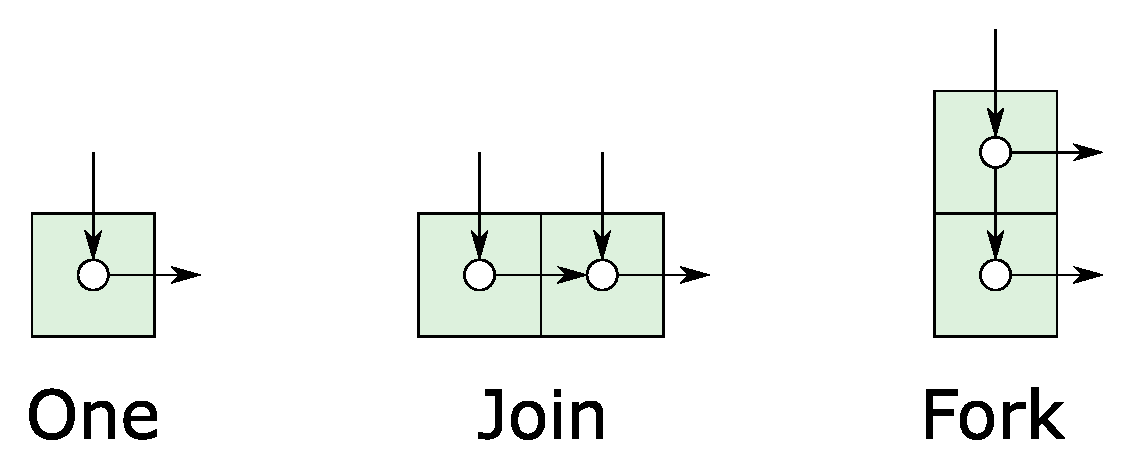
\includegraphics[width=0.4\textwidth]{images/one-join-fork.pdf}
    \caption{One-Join-Fork matrix constructors. \label{fig:one-join-fork}}
\end{figure}
Here \hs{One} is the inductive base case that construct the \emph{one-element} matrix; \hs{Join} and \hs{Fork} are the two basic binary constructors available for building matrices out of other matrices as you can see in Fig.~\ref{fig:one-join-fork}.

These simple four constructors provide a type safe inductive definition where it is not possible to construct a malformed matrix such as \[\hs{Matrix { matrix = [[1,0],[0,1]], dimensions = (4,4) }}\] for example.

The trick is to define a recursive data type in which dimensions are typed by algebraic data types and use a GADT in order to control the output type dimensions and maintain the \hs{Join} and \hs{Fork} dimension invariants across the data structure.

\subsection{Constructing matrices}

This solution was built on the notion that algebraic data types are isomorphic to their cardinality, e.g. |\hs{Void}| $ \cong 0$, |\hs{()}| $\cong 1$, |\hs{Either a b}| $\cong |a| + |b|$ and so on. Furthermore, this GADT guarantees that a matrix will always have valid dimensions, i.e. is type-correct by construction. For instance, the $2 \times 2$ identity matrix
%
$\begin{aligned}
\begin{bmatrix}
\left.\begin{matrix}
\dfrac{1}{0}
\end{matrix}\ \right|\ \begin{matrix}
\dfrac{0}{1}
\end{matrix}
\end{bmatrix}
\end{aligned}{}$ can be expressed by:
\vspace{1mm}
\begin{minted}[xleftmargin=10pt]{haskell}
iden2x2 :: Num e 
        => Matrix e (Either () ()) (Either () ())
iden2x2 = Fork (Join (One 1) (One 0)) 
               (Join (One 0) (One 1))
\end{minted}
\vspace{1mm}

For larger matrices, declaring type signatures by hand becomes troublesome. So, two type families were created to make it easier to work with matrix dimension definition:

\vspace{1mm}
\begin{minted}[xleftmargin=10pt]{haskell}
type family Count (d :: Type) :: Nat where
  Count Void         = 0
  Count ()           = 1
  Count (Either a b) = (+) (Count a) (Count b)
  Count (a, b)       = (*) (Count a) (Count b)
  -- Generics
  -- (...)
  
type family FromNat (n :: Nat) :: Type where
  FromNat 0 = Void
  FromNat 1 = ()
  FromNat n = FromNat' (Mod n 2 == 0) 
                       (FromNat (Div n 2))

type family FromNat' (b :: Bool) (m :: Type) where
  FromNat' 'True m  = Either m m
  FromNat' 'False m = Either () (Either m m)
\end{minted}
\vspace{1mm}

The purpose of the \hs{Count} type family will be used to compute the normalised dimension types, as will be seen in \S\ref{subsec-newtype-wrappers}. If one wants to be able to have matrix typed by generic arbitrary data types (as we'll see in \S\ref{sec-appl}), one needs to add support for generic types. We leave the trivial implementation out of the \doc\ for simplicity. The \hs{FromNat} type family builds a balanced tree of \hs{Either}s at the type-level, from a type-level natural, that is supposed to be the matrix dimension.

These type families take advantage of the algebraic data type cardinality isomorphism and provide a conversion mechanism \emph{from} and \emph{to} data types/type-level naturals. So the same $2 \times 2$ identity matrix can now be defined as:

\vspace{1mm}
\begin{minted}[xleftmargin=10pt]{haskell}
iden2x2 :: Num e => Matrix e (FromNat 2) (FromNat 2)
iden2x2 = Fork (Join (One 1) (One 0)) 
               (Join (One 0) (One 1))
\end{minted}
\vspace{1mm}

Notice that type families can be seen as type-level functions that are called at compile-time. So a type-level demanding program will take longer to compile, specially if it declares several large matrices. Thankfully, \hs{FromNat} takes advantage of the possibility of reducing the number of computations needed to calculate the normalised dimension type that provides a significant speedup.

\section{Matrix manipulation and transformation} \label{sec:200303a}

The proposed inductive matrix data type enables the use of pattern matching and the laws of the linear algebra of programming (\S\ref{laop-laws}) to write total, efficient and statically typed manipulation and transformation functions. In view of this, matrix composition (\emph{aka} matrix-matrix multiplication) can be defined elegantly and in a more calculational way, in contrast with the partial, (ugly) low-level nested for-loop implementation, which can be found in most imperative languages:
\begin{minted}[xleftmargin=10pt]{haskell}
comp :: Num e => Matrix e cr rows 
     -> Matrix e cols cr -> Matrix e cols rows
comp (One a) (One b)       = One (a * b)
comp (Join a b) (Fork c d) = comp a c + comp b d
comp (Fork a b) c          = 
    Fork (comp a c) (comp b c)
comp c (Join a b)          = 
    Join (comp c a) (comp c b)
\end{minted}
Like matrix multiplication, other common operations, such as matrix transposition, benefit from a block-oriented structure that leads to a simple and natural divide-and-conquer algorithmic solution. Performance wise, this means that without much effort we can obtain optimal cache-oblivious algorithms\footnote{A cache-oblivious algorithm is such that no variables that depend on hardware parameters, such as the size of the cache and the length of the cache-line, need to be tuned to achieve optimality.} \citep{frigo1999cache}. The basic philosophy in designing a cache-oblivious algorithm is to use a recursive approach that repeatedly divides the data-set until it eventually becomes cache resident and thus cache optimal, as we can see from the definition of the \hs{comp} function above.

In the type-class mechanics of Haskell \cite{hall1996type}, matrix entry-wise addition, multiplication and subtraction fit nicely by defining a \hs{Num} instance, as well as entry-wise matrix comparison and equality, by defining \hs{Ord} and \hs{Eq} instances, respectively. Sadly, there are no fusion laws that help defining an appropriate inductive definition of matrix equality when the two matrices have different valid permutations of \hs{Join}s and \hs{Fork}s, for example. This can still be done, however, by taking advantage of the exchange (``\emph{abide}") law (\ref{abide-law}):

\vspace{1mm}
\begin{minted}[xleftmargin=10pt, mathescape=true]{haskell}
-- Abide Join-Fork
abideJF :: Matrix e cols rows -> Matrix e cols rows
abideJF (Join (Fork a c) (Fork b d)) = 
    Fork 
        (Join (abideJF a) (abideJF b)) 
        (Join (abideJF c) (abideJF d))
abideJF (One e)    = One e
abideJF (Join a b) = Join (abideJF a) (abideJF b)
abideJF (Fork a b) = Fork (abideJF a) (abideJF b)

instance Eq e => Eq (Matrix e cols rows) where
  (One a) == (One b)           = a == b
  (Join a b) == (Join c d)     = a == c && b == d
  (Fork a b) == (Fork c d)     = a == c && b == d
  x@(Fork _ _) == y@(Join _ _) = x == abideJF y
  x@(Join _ _) == y@(Fork _ _) = abideJF x == y
\end{minted}
\vspace{1mm}

It is worth noting that one major downside of this encoding is that \hs{Either (Either () ()) ()} is different from \hs{Either () (Either () ())}, for example, even though both represent $3$. This implies that two matrices with the same dimension can have different types, and thus, for example, they can not be tested for equality. One way to address this downside is shown in \S\ref{subsec-newtype-wrappers}, by introducing a new-type matrix wrapper with generic arbitrary dimensions. Another approach is to manually write an identity matrix that exposes this isomorphism and use it to obtain a matrix of the same dimensions.  

\section{Matrix construction}\label{l-m-s}

It is not possible to construct typed matrices depending on the type of the dimensions desired, because GHC is not able to infer the correct GADT types. One way to achieve this is by using type-classes. Type-classes can be seen as functions from types to values and they are the solution for writing methods that allow building matrices from other representations (e.g.\ list of lists of elements) in the same inductive way, as is the case of class \hs{FromLists}.
\begin{minted}[xleftmargin=10pt, mathescape=true]{haskell}
class FromLists e cols rows where
  fromLists :: [[e]] -> Matrix e cols rows
\end{minted}
\noindent %Please note that is only possible to implement a version of 
Note that \hs{fromLists} can fail at run-time if the input list is not complacent with the desired matrix dimensions. It is possible to offer wrapper functions around it that guarantee it won't fail at compile time.
%However, an alternative way of building matrices from other representations, that is fully type-safe, exists thanks to the linear map semantics of matrices, although we leave this out of the scope of the \doc.

%As is well-known, matrices are a way to represent linear transformations on vectors. So, by defining the semantics of the \hs{Matrix} type as vector-to-vector map, this can be used to define construction and deconstruction functions in a fully type-safe way. Below we briefly show how to implement a total, fully type-safe and polymorphic matrix construction function, using this approach. Vectors and linear maps can be represented by the following types, respectively:
%
%\vspace{1mm}
%\begin{minted}[xleftmargin=10pt]{haskell}
%newtype Vector e a = Vector { at :: a -> e }
%
%type LinearMap e a b = Vector e a -> Vector e b
%\end{minted}
%\vspace{1mm}
%
%The \hs{Vector} type can be easily instantiated in classes \\\hs{Contravariant} and \hs{Num} (details omitted for economy of space). The semantic interpretation function can then be defined as follows:
%
%\vspace{1mm}
%\begin{minted}[xleftmargin=10pt]{haskell}
%semantics :: Num e => Matrix e a b -> LinearMap e a b
%semantics m = case m of
%  Empty    -> id
%  One e    -> const (Vector (const e))
%  Join x y -> 
%    \v -> semantics x (Left >$< v) 
%          + semantics y (Right >$< v)
%  Fork x y -> 
%    \v -> Vector $ either (at (semantics x v)) 
%                          (at (semantics y v))
%\end{minted}
%\vspace{1mm}
%
%This function converts a \hs{Matrix} into a \hs{LinearMap}. With this new representation, matrix deconstruction algorithms can be written in a relatively straightforward way. However, the other way around is only achievable via type-classes, as noted above.
%
%\vspace{1mm}
%\begin{minted}[xleftmargin=10pt]{haskell}
%class Construct a where
%  row :: Num e => Vector e a -> Matrix e a ()
%  linearMap :: (Construct b, Num e) 
%            => LinearMap e a b -> Matrix e a b
%\end{minted}
%\vspace{1mm}
%
%By instantiating the type-class above for the inductive cases of \hs{a = ()} and \hs{a = Either a b} and with the help of a simple helper function, one obtains a total, fully type-safe \hs{matrixBuilder} function:\footnote{The implementation details can be found in the following link: \url{https://tinyurl.com/xxxx} NB: name removed for the sake of anonymity.}%\url{https://tinyurl.com/rexm92k}.}

%\vspace{1mm}
%\begin{minted}[xleftmargin=10pt]{haskell}
%type Constructable a b = (Construct a, Construct b)
%type Enumerable a = (Enum a, Bounded a)
%
%dot :: (Num e, Enumerable a) 
%    => Vector e a -> Vector e a -> e
%dot x y = 
%    sum [at x a * at y a | a <- [minBound..maxBound]]
%
%matrixBuilder :: 
%              (Num e, Constructable a b, Enumerable a) 
%              => ((a, b) -> e) -> Matrix e a b
%matrixBuilder f = 
%    linearMap $ \v -> 
%        Vector $ \b -> 
%            dot v $ Vector $ \a -> f (a, b)
%\end{minted}
%\vspace{1mm}
%
%This linear map semantics can be used for other programming purposes. However,
%%is important to realise that it is not necessary to go via linear maps for interpreting a matrix. 
%algorithms defined directly over the inductive structure tend to be more efficient, see \S \ref{subsec-bench}.
%%an very efficient way however, linear maps can be more straightforward to work with than the inductive data type in some cases, but are less efficient.

\section{Category instance}\label{sec:cat}

In \S\ref{sec-intro} we showed how matrices form a category where objects are dimensions and morphisms are the matrices themselves.

The proposed inductive structure arranges its type parameters in order to be able to provide a type-class instance for \hs{Category}. It helps the end-user to make better use of code and reason about it, by using more readable notation and by allowing the compiler to infer which type-class instances to use. Throughout the rest of the paper we will use \hs{id} and \hs{(.)} interchangeably to mean either function or matrix composition/identity.

Given that the \hs{iden}tity matrix needs certain type constrains on the dimension types, only a constrained version of the \hs{Category} type-class can be offered.\footnote{Note that this limitation also happens when trying to implement idiomatic instances of the \hs{Functor} hierarchy in Haskell.
%nonetheless, equivalent definitions are in reach.
} In this context, the following instance is given:
%so that the users can read (reason about) code more easily:

\vspace{1mm}
\begin{minted}[xleftmargin=10pt]{haskell}
class Category k where
    type Object k o :: Constraint
    type Object k o = ()
    id :: Object k a => k a a
    (.) :: k b c -> k a b -> k a c
    
instance Category (Matrix e) where
    type Object (Matrix e) a =
        (FromLists e a a, Countable a)
    id = iden
    (.) = comp
\end{minted}
\vspace{1mm}
Note that \hs{Countable = KnownNat (Count a)}.

\section{End-user interface}\label{sec-manipulation}

As one can imagine, working with very large matrices at the type level can be an unpleasant experience. This section presents two new-type wrappers around the canonical data type that aim to improve end-user interfacing, also giving an overview of the available library API and how error messages look like when using the generalised dimensions wrapper.

\subsection{Matrix new type wrappers}\label{subsec-newtype-wrappers}

It is possible to abstract the use of the \hs{FromNat} type family, obtaining a new-type matrix wrapper which dimensions are type level naturals (provided by the TypeLits library). 

\vspace{1mm}
\begin{minted}[xleftmargin=10pt, mathescape=true]{haskell}
import qualified Matrix.Internal as I

newtype Matrix e (cols :: Nat) (rows :: Nat) = 
    M (I.Matrix e 
        (I.FromNat cols)
        (I.FromNat rows))
\end{minted}
\vspace{1mm}

Thanks to the type family defined below, it is possible to attain a matrix typed by arbitrary generic data types. This will be the new type wrapper used throughout the rest of the \doc.

\vspace{1mm}
\begin{minted}[xleftmargin=10pt, mathescape=true]{haskell}
type family Normalize (d :: Type) :: Type where
  Normalize (Either a b) = Either (Normalize a)
                                  (Normalize b)
  Normalize d            = FromNat (Count d)

newtype Matrix e (cols :: Type) (rows :: Type) = 
    M (I.Matrix e 
        (I.Normalize cols) 
        (I.Normalize rows)) 
\end{minted}
\vspace{1mm}

\hs{Normalize} needs to preserve the \hs{Either}-based structure to comply with the type signature of \hs{Join} and \hs{Fork}, balancing the tree in all other cases.

This new-type captures the matrix type generalisation proposed by \citet{oliveira2012towards}. In short, objects in categories of matrices can be generalised from numeric dimensions ($n, m \in \mathbb{N}_0$) to arbitrary denumerable types $(A,B)$, taking disjoint union $A + B$ for $m + n$, Cartesian product $A \times B$ for $m \times n$, unit type $()$ for number $1$, etc.

\subsection{Algebra of Programming API}\label{sec:api}

The \hs{Matrix} data type and the aforementioned new-type wrappers are a part of the LAoP programming library developed in Haskell.\footnote{LAoP stands for ``Linear Algebra of Programming".} This library provides an API for construction and manipulation of these types. The API offers the main combinators of the linear algebra of programming wherefrom other linear algebra operations can be derived.

Listing \ref{lst:api} presents the set of most important function signatures that are part of the generalised dimensions module API.
\begin{listing*}
\begin{minted}[xleftmargin=10pt, mathescape=true, fontsize=\small]{haskell}
one            :: e -> Matrix e () () -- Unit constructor
join           :: Matrix e a r -> Matrix e b r -> Matrix e (Either a b) r -- Join constructor
fork           :: Matrix e c a -> Matrix e c b -> Matrix e c (Either a b) -- Fork constructor
matrixBuilder  :: (...) => ((a, b) -> e) -> Matrix e a b                  -- Builder function
fromF          :: (...) => (a -> b) -> Matrix e a b                       -- Lifts functions
point          :: (...) => a -> Matrix e () a                             -- Point vector
comp           :: Num e => Matrix e cr r -> Matrix e c cr -> Matrix e c r -- Composition (MMM)
(.|)           :: Num e => e -> Matrix e c r -> Matrix e c r         -- Scalar multiplication
(./)           :: Fractional e => Matrix e c r -> e -> Matrix e c r  -- Scalar division
iden           :: (...) => Matrix e c c             -- Identity matrix
tr             :: Matrix e c r -> Matrix e r c      -- Transposition
abideJF        :: Matrix e c r -> Matrix e c r      -- Join-Fork exchange
abideFJ        :: Matrix e c r -> Matrix e c r      -- Fork-Join exchange
p1             :: (...) => Matrix e (Either m n) m  -- First projection
p2             :: (...) => Matrix e (Either m n) n  -- Second projection
i1             :: (...) => Matrix e m (Either m n)  -- First injection
i2             :: (...) => Matrix e n (Either m n)  -- Second injection
fstM           :: (...) => Matrix e (m, k) m  -- Pairing first projection
sndM           :: (...) => Matrix e (m, k) k  -- Pairing second projection
kr             :: (...) => Matrix e c a -> Matrix e c b -> Matrix e c (a, b)
               -- Pairing (Khatri-Rao Product)
(-|-)          :: (...) => Matrix e n k -> Matrix e m j -> Matrix e (Either n m) (Either k j) 
               -- Co-product bi-functor (Direct Sum)
(><)           :: (...) 
               => Matrix e m p -> Matrix e n q -> Matrix e (m, n) (p, q)
               -- Product bi-functor (Kronecker)
\end{minted}
\caption{LAoP API}
\label{lst:api}
\end{listing*}{}
\noindent As an example of using this API to write matrix operations by composing functions, the following function provides a \hs{join}/\hs{fork} version of matrix entry-wise addition, where \hs{(-|-)} can be seen as the matrix direct sum operation:
{\small
\begin{minted}[xleftmargin=10pt, mathescape=true]{haskell}
addition :: (...) => Matrix e cols rows 
         -> Matrix e cols rows -> Matrix e cols rows
addition a b =
    (join id id) . (a -|- b) . (fork id id)
\end{minted}
}
\noindent This expresses the relationship between the underlying additive operator and direct sum. The correctness of \hs{addition} is granted by the absorption law (\ref{eq:101221f}), among others:
\small
\begin{eqnarray*}
\start
    \hs{(join id id) . (a -|- b) . (fork id id)}
\just={ absorption law (\ref{eq:101221f}) ; identity (\ref{eq-id})}
    \hs{(join a b) . (fork id id)}
\just={ divide-and-conquer - (\ref{eq-divide-and-conquer}); identity (\ref{eq-id})}
    \hs{(a + b)}
\end{eqnarray*}
\normalsize

Note that all the combinators on dimension types are polymorphic. This is a feature that does not exist or is rather fragile in other programming matrix libraries. However, the expected type constraints and type-level mechanisms (type-level natural and type-families) that make the type polymorphism work can make the type-signatures convoluted. For space economy, these are omitted from the above-mentioned API and throughout the \doc. Nonetheless, this downside is minimised by providing a set of aliases of type in order to reduce the length and improve the readability and, in some cases, reasoning of the required restrictions. For illustrative purposes, we give the full type signature of the \hs{addition} function presented above with and without the syntactic sugar:

\begin{minted}[xleftmargin=10pt, mathescape=true]{haskell}
addition :: 
  (Num e, FromLists c c, FromLists m m,
   KnownNat (Count c),  KnownNat (Count m)) 
  => Matrix e m c -> Matrix e m c  -> Matrix e m c

addition :: 
  (Num e, FL c c, FL m m, CountableDims c m)
  => Matrix e m c -> Matrix e m c  -> Matrix e m c
\end{minted}

When doing type-level programming error messages easily become cumbersome and hard to read. By using typed matrices and a strongly typed language most dimension check errors can be caught at compile time. However, if the error messages are not clear, this fact does not impose any benefit. Gladly, error messages in our library do not suffer from the type-level machinery involved as we can see from the simple example, where we try to join two matrices with different row types:

\begin{minted}[xleftmargin=10pt, mathescape=true]{haskell}
-- x :: Matrix Float Bool Bool
-- y :: Matrix Float Bool Ordering
error:
- Couldn't match type 'Ordering' with 'Bool'
Expected type: Matrix Float Bool Bool
Actual type: Matrix Float Bool Ordering
- In the second argument of 'join', namely 'y'
In the expression: join x y
In an equation for 'it': it = join x y
\end{minted}

The matrix programming library developed in the scope of this paper can be found in the Hackage repository along with its API documentation\footnote{
\url{https://hackage.haskell.org/package/laop}}.
%\url{https://hackage.haskell.org/package/xxxxx/}. NB: package name removed for the sake of anonymity.}.

\section{Equational reasoning}\label{sec-eq-reas}

This section shows how to use equational reasoning and the laws of the linear algebra of programming to prove properties of functions on matrices and/or to obtain more efficient programs.
% For example, to prove that:
%	\vspace{1mm}
%	\begin{minted}[xleftmargin=10pt, mathescape=true]{haskell}
%	(Join a b) . (c -|- d) == Join (a . c) (a . d)
%	\end{minted}
%	\vspace{1mm}
%	Where \hs{(.) = comp}. The left-hand side is rewritten using the functions definitions:
%	\begin{eqnarray*}
%	\start
%	    \hs{(Join a b) . (c -|- d)}
%	\just={ \hs{(-|-)}'s definition }
%	    \hs{(Join a b) . (Join (i1 . c) (i2 . d))}
%	\just={\hs{Join}'s fusion - (\ref{fusion-join})}
%	    \hs{Join ((Join a b) . (i1 . c)) ((Join a b) . (i2 . d))}
%	\just={Cancellation - (\ref{cancel-join})}
%	    \hs{Join (a . c) (b . d)}
%	\end{eqnarray*}
%	Proving

A good example of this is the \hs{select} operator inspired by the \hs{Selective} interface. Selective Functors are a recent abstraction in functional programming. The argument in favour of these Selective Functors advocates them as solving the limitation of Applicatives and Monads in the context of static analysis, allowing over-approximation and under-approximation of effects in a circuit with conditional branches \cite{andrey2019selective}. From a linear algebra perspective, this abstraction allows the study of conditional probability calculations when dealing with left stochastic matrices \cite{Armando2020}. 

\begin{wrapfigure}[6]{r}{11em}
\vskip -2em \begin{tikzcd}[column sep=small]
&&
	b
\\
	a \arrow[rr, "i_1"]
          \arrow[rru, "y", bend left]
&&
	a + b \arrow[u, "{[ y\ |\ id]}"']
&&	b \arrow[ll, "i_2"']
          \arrow[llu, "id"', bend right]
\\
&&
	c \arrow[u, "m"']
\end{tikzcd}
\end{wrapfigure}
From an abstract point-of-view, the diagram alongside corresponds to the \hs{ArrowChoice} implementation of \hs{select} where, in the case of stochastic matrices, \hs{m} can be seen as a probability distribution that outputs either \hs{a} or \hs{b}, and \hs{y} is only computed for values of type \hs{a}, all others are skipped.

This leads to a straightforward implementation of \hs{select} in terms of matrices:
\begin{minted}[xleftmargin=10pt, mathescape=true]{haskell}
select :: (...) => Matrix e c (Either a b) 
       -> Matrix e a b -> Matrix e c b
select m y = join y id . m
\end{minted}
We know upfront from the definition that a (possibly) expensive computation is taking place where one of the matrices is the \hs{id}entity. But, from the type of \hs{m} we know that it can be \hs{m = Fork x z} for some \hs{x} and \hs{z} (\ref{eq:091206c}) and the implementation can take advantage of this: \small
\begin{eqnarray*}
\start
    \hs{join y id . m}
\just={\hs{m = Fork x z}}
    \hs{join y id . Fork x z}
\just={ divide-and-conquer (\ref{eq-divide-and-conquer}) }
    \hs{y . x + id . z}
\just={ identity law (\ref{eq-id}) }
    \hs{y . x + z}
\end{eqnarray*}\normalsize
Thus one gets
\begin{minted}[xleftmargin=10pt, mathescape=true]{haskell}
select (Fork x z) y = y . x + z
\end{minted}
gaining in efficiency because \hs{x} is necessarily smaller than the original \hs{m}.
% was used to find a way to compute the result more directly, and therefore more efficiently.
Note that \hs{x} and \hs{z} above can be, on their own, joins. In this case, by the abide law (\ref{abide-law}) one gets \\\hs{m = Join (Fork x c) (Fork z d)} which lets us pattern match one level deeper and, benefiting from the divide-and-conquer law, end up with: \small
\begin{eqnarray*}
\start
    \hs{join y id . m}
\just={\hs{m = Join (Fork x c) (Fork z d)}}
    \hs{join y id . Join (Fork x c) (Fork z d)}
\just={ fusion (\ref{fusion-join}) }
    \hs{Join (join y id . Fork x c) (join y id . Fork z d)}
\just={ divide-and-conquer (\ref{eq-divide-and-conquer}) twice; identity (\ref{eq-id}) twice }
    \hs{Join (y . x + c) (y . z + d)}
\end{eqnarray*}\normalsize

%By further pattern matching on \hs{m}, it may be the case \hs{m = Join x z} it is possible to benefit from linear algebra laws again and reduce the complexity of this operator even further: in the case of \hs{m = Join x z},
%\begin{equation}\label{eq-join-reas}
%\begin{array}{rcl}
%\start
%    \hs{join y id . Join x z}
%\just={\hs{Join}'s fusion law}
%    \hs{Join (join y id . x) (join y id . z)}
%\end{array}
%\end{equation}
%This is not very interesting because \hs{id} is still there but, if we pattern match one level deep we can benefit from the divide-and-conquer-law and end up with:

\noindent Putting everything together, one gets the following more efficient implementation:
\begin{minted}[xleftmargin=10pt, mathescape=true]{haskell}
select :: (...) => Matrix e c (Either a b) 
       -> Matrix e a b -> Matrix e c b
select (Fork x z) y                   = y . x + z
select (Join (Fork x c) (Fork z d)) y = 
    join (y . x + c) (y . z + d)
select m y                            = 
    join y id . m
\end{minted}
By exploring linear algebra properties, the compiler can actually be instructed to optimise the program by defining correct rewrite rules \cite{jones2001playing}. GHC's rewrite rules allow the programmer to directly communicate to the compiler ways of optimising a program that is not obvious to it, for instance:
\begin{minted}[xleftmargin=10pt, mathescape=true]{haskell}
{-# RULES 
   "prod/cancel1" forall a b. p1 . (fork a b) = a;
   "co-p/cancel1" forall a b. (join a b) . i1 = a;
#-}
\end{minted}
This tells the compiler to skip computations wherever it encounters an instance of the cancellation laws (\ref{cancel-join},\ref{cancel-fork}).
% but, the linear algebra of programming is full of
Other useful laws such as converse duality (\ref{converse-duality}) or fusion (\ref{fusion-join},\ref{fusion-fork}) can be used for the same purpose. In possession of such rules, the compiler becomes aware of possible non trivial optimisations and applies a certain degree of equational reasoning to produce more efficient code.

%Practical results and benchmarks of the transformations presented in this section can be found in section \ref{subsec-bench}.

\section{Applications and benchmarks}\label{sec-appl}
This section starts by giving two simple examples of application of the LAoP library.

%\subsection{Linear Algebra Semantics of Spreadsheets}\label{subsec-laop}
%
%\citet{COS20} present a formal semantics for spreadsheets (SS) based on typed linear algebra (LA). Below we show how such semantics can be expressed in the library presented in this paper\footnote{The project is to design a static SS analyser automating such a conversion from Gnumeric XML sources.} through a simple example, shown in the figure below. This depicts a typical SS containing some students' marks. There are cells filled with numbers and cells filled with strings. Some cells displaying numbers are actually formul\ae\ involving 
%other cells (e.g.\ those of columns \textsf{Exam} and \textsf{Final}):
%\begin{figure}[H]
%    \centering
%	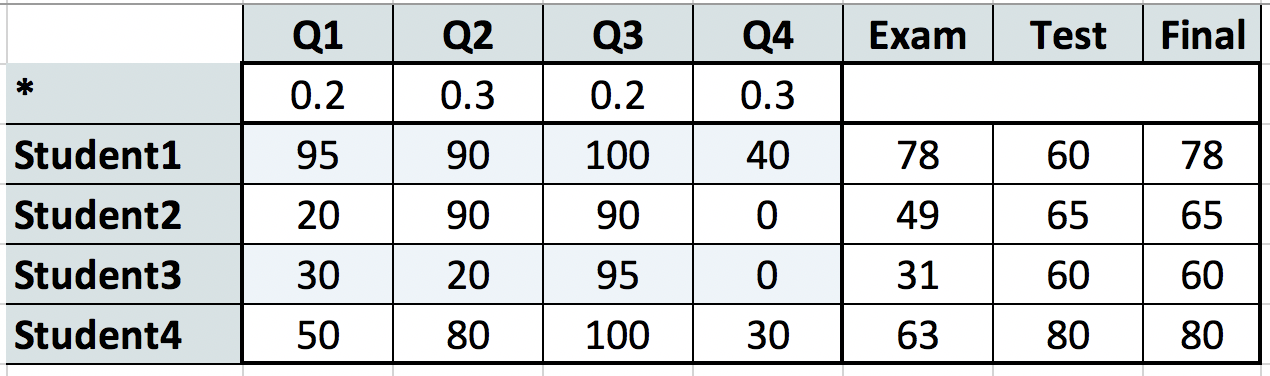
\includegraphics[width=.45\textwidth]{images/students.png}
%    \label{fig:students}
%\end{figure}{}
%The typed LA semantics of this spreadsheet regards rectangles of numbers as \emph{source} (data) matrices and those containing formul\ae\ as matrices too, but linked to the former by semantic constraints. Cells containing strings (displayed in grey in the SS) are regarded as \emph{type} elements. There are three types in the given SS,
%%\begin{eqnarray*}
%%\start Student = \{Student1 .. Student4\}
%%\more  Question = \{ Q1 .. Q4 \}
%%\more  Results = \{ Exam, Test, Final \}
%%\end{eqnarray*}
%\begin{minted}[xleftmargin=10pt, mathescape=true]{haskell}
%data Student = Student1 | Student2 
%             | Student3 | Student4
%  deriving (Eq, Show, Enum, Bounded, Generic)
%
%data Question = Question1 | Question2 
%              | Question3 | Question4
%  deriving (Eq, Show, Enum, Bounded, Generic)
%
%data Results = Exam | Test | Final
%  deriving (Eq, Show, Enum, Bounded, Generic)
%\end{minted}
%
%\begin{wrapfigure}[6]{r}{16em}
%\centering \vskip -0.5em \(
%\xymatrix{
%	Question
%		\ar[r]^{m}
%		\ar[d]_{\omega}
%&
%	Student
%		\ar[dl]_-{\tau}
%&
%	Results
%		\ar[l]_{r}
%\\
%	()
%		\ar[rru]_{~~~exam, test, final}
%}
%\)
%\end{wrapfigure}
%\noindent and the matrices and vectors typed by them given in the diagram alongside. Note that arrows in the diagram depict matrices.
%
%Row vector $\omega$ records the weights associated to the questions, \hs{m} is the marks matrix (ranging over the interval \hs{[0..100]}), \hs{r} is the results matrix and \hs{exam} is a column vector representing the \hs{Exam} \emph{point}\footnote{\emph{Points} are functions of type \hs{() -> A} (therefore constant functions), which \hs{fromF} converts into column vectors. See e.g.\ \hs{point} in the API of \S\ref{sec:api}.} and similarly for the other inhabitants of \hs{Results}. (That is, \hs{exam}, \hs{test}, \hs{final} form the standard basis of the \hs{Results}-dimensional vector space.)
%
%The perspective of \citet{COS20} is that, while string-valued cells in a SS represent types, areas with numbers only --- which users can change at their will --- are regarded as parameter matrices of the SS. Finally, cells holding formul\ae\ 
%express the SS functional behaviour, at matrix-level. Following this view,
%the formal semantics of the student marks' SS given above is the matrix-valued function
%\begin{eqnarray}
%xls\ \ \omega\ m \ \tau = \matfour \omega 0 m r
%\end{eqnarray}
%where result matrix $r$ is given by the matrix sum:
%\begin{eqnarray*}
%	{r} =& {M} \comp \conv{\omega} \comp \conv{exam}
%		\mathbin{+}
%	\conv{\tau} \comp \conv{test}
%		\mathbin{+}
%	\\&({r} \comp test) \mathbin{`{max}`}(r \comp exam) \comp \conv{final}
%\end{eqnarray*}
%
%The first term purports the semantics of calculating the exam marks as a weighted sum; the second places the marks of a previous test $\tau$ in the \hs{Test} column; and finally the third summand takes the entry-wise maximum of the exam and test vectors. 
%Altogether, using block matrix typing % --- recall (\ref{eq:xxxx}) -- 
%we infer that the type of the output of \ensuremath{{xls}} is 
%\begin{quote}
%\ensuremath{{Question}\mathbin{+}{Results}\to \mathrm{()}\mathbin{+}{Student}}.
%\end{quote}
%Thus the overall type of the spreadsheet is:
%\begin{eqnarray*}
%xls &::& (Question \to ()) \to
%\more (Question \to Student) \to
%\more (Student \to ()) \to
%\more (Question + Results \to () + Student)
%\end{eqnarray*}
%or in Haskell notation:
%\begin{minted}[xleftmargin=10pt, mathescape=true]{haskell}
%xls :: Matrix Float Question One
%    -> Matrix Float Question Student
%    -> Matrix Float Student One
%    -> Matrix Float (Either Question Results) 
%                    (Either One Student)
%\end{minted}

\subsection{Probabilistic programming} \label{subsec-prob-laop}
Probabilistic programming arises naturally from functional programming once we replace ``sharp" functions by probabilistic ones, represented by stochastic matrices, also known as Markov chains \cite{oliveira2012towards}. Let us show this taking an example from the \citet{wiki:BayesianNetwork}. Suppose we define the following predicates modelling the behaviour of a sprinkler, where \hs{S} (sprinkler on/off), \hs{R} (raining or not) and \hs{G} (grass wet or not) are Booleans:
\begin{eqnarray*}
\begin{array}{rcl}
\start\hs{sprinkler :: R -> S}
\more\hs{sprinkler r = not r}
\end{array}
\begin{array}{rcl}
\start\hs{grass :: (S, R) -> G}
\more\hs{grass (s,r) = s || r}
\end{array}
\end{eqnarray*}
The second predicate tells that the grass will be wet if and only if either it is raining or the sprinkler is on. The first tells that the sprinkler is on \emph{iff} it is not raining. Composing these two predicates we see that rain completely determines the state of the grass:
\begin{eqnarray*}
%\start grass\ (sprinkler\ r,r) = \neg r \vee r = True
\start \hs{grass (sprinkler s, rain) = not rain || rain} 
\more \therefore \hs{True}
\end{eqnarray*}

\begin{wrapfigure}[09]{r}{7em}
\vskip -1em\(
\xymatrix@R=1.3em{
	(G, (S, R))
\\
	(S, R)
		\ar[u]_{grass \kr id}
\\
	R
		\ar[u]_{sprinkler \kr id}
\\
	()
		\ar[u]_{rain}
}
\)
\end{wrapfigure}
Looking at the diagram alongside, where \hs{(}$\kr$\hs{)} can be seen as equal to \hs{(&&&)}\footnote{From \hs{Control.Arrow}, specialised to \hs{(->)}}, we see that the system has two possible states in \hs{(G, (S, R))}
--- either \hs{(True, (True, False))} or \hs{(True, (False, True))} ---
the grass being wet in both. So it will melt because of being wet all the time.

Clearly, this deterministic interpretation of the diagram does not correspond to reality, but its stochastic interpretation will do. For this, we just need to regard the arrows as denoting stochastic matrices and not pure functions, for instance\footnote{For easy reference we follow the Wikipedia example closely.}
\begin{eqnarray*}
\start \longrarrow R {sprinkler} S = \matfour{0.60}{0.99}{0.40}{0.01}
\more \rarrow{(S, R)} {grass} G =
\begin{bmatrix}
    1.00    & 0.20    & 0.10    & 0.01 \\
    0    &    0.80    & 0.90    & 0.99
\end{bmatrix}
\end{eqnarray*}
This describes a probabilistic system \emph{reactive} to the rain. Once its distribution becomes known, eg.
\begin{eqnarray*}
\rarrow 1 {rain} R = \begin{bmatrix} 0.80 \\ 0.20 \end{bmatrix}
\end{eqnarray*}
one immediately gets the distribution of the overall state, given by column vector \small
\begin{eqnarray}
\rarrow 1 {state} {(G, (S, R))} &=~~~~& 
\begin{array}{rrrr}
G  	& S  	& R 	&        \\\hline
\multirow{4}{*}{dry}	& \multirow{2}{*}{off}	& no	& 0.4800 \\\cline{3-3}
	& 	& yes	& 0.0396 \\\cline{2-3}
	& \multirow{2}{*}{on}	& no	& 0.0320 \\\cline{3-3}
	& 	& yes	& 0.0000 \\\cline{1-3}
\multirow{4}{*}{wet}	& \multirow{2}{*}{off}	& no	& 0.0000 \\\cline{3-3}
	& 	& yes	& 0.1584 \\\cline{2-3}
	& \multirow{2}{*}{on}	& no	& 0.2880 \\\cline{3-3}
	& 	& yes	& 0.0020 \\\cline{1-4}
\end{array} \label{eq:state}
\\\nonumber
\end{eqnarray} \normalsize
which is calculated following the diagram. Consider the following matrices
\vskip 1ex
\begin{minted}[xleftmargin=10pt, mathescape=true]{haskell}
rain :: Matrix Prob () R
sprinkler :: Matrix Prob R S
grass :: Matrix Prob (S, R) G
\end{minted}
\vskip 1ex
(where \hs{type Prob = Double})
encoded in the LAoP library, where we also free the types involved from the strict Boolean model, already visible in (\ref{eq:state}).\footnote{So, instead of \hs{G = Bool}, we have the more descriptive \hs{G = Dry | Wet} and so on.}
%\vskip 1ex
%\begin{minted}[xleftmargin=10pt, mathescape=true]{haskell}
%type Prob = Double
%
%rain :: Matrix Prob () R
%rain = matrixBuilder gen
%  where
%    gen (_, No)  = 0.8
%    gen (_, Yes) = 0.2
%
%sprinkler :: Matrix Prob R S
%sprinkler = matrixBuilder gen
%  where
%    gen (No, Off)  = 0.6
%    gen (No, On)   = 0.4
%    gen (Yes, Off) = 0.99
%    gen (Yes, On)  = 0.01
%
%grass :: Matrix Prob (S, R) G
%grass = matrixBuilder gen
%  where
%    gen ((Off, No), Dry)  = 1
%    gen ((Off, Yes), Dry) = 0.2
%    gen ((On, No), Dry)   = 0.1
%    gen ((On, Yes), Dry)  = 0.01
%    gen ((Off, No), Wet)  = 0
%    gen ((Off, Yes), Wet) = 0.8
%    gen ((On, No), Wet)   = 0.9
%    gen ((On, Yes), Wet)  = 0.99
%\end{minted}
%\vskip 1ex
The distribution of the overall state displayed above
is given by the expression
\vskip 1ex
\begin{minted}[xleftmargin=10pt, mathescape=true]{haskell}
state = compose grass sprinkler rain
\end{minted}
\vskip 1ex
where
\begin{minted}[xleftmargin=10pt, mathescape=true]{haskell}
compose :: (...) 
        => Matrix e (c, d) b
        -> Matrix e d c
        -> Matrix e a d
        -> Matrix e a (b, (c, d))
compose g s r = tag g . tag s . r

tag :: (...) => Matrix e a b -> Matrix e a (b, a)
tag f = kr f id
\end{minted}
\vskip 1ex
Note the role of the $tag$ operation, which for functions amounts to \hs{tag f x = (f x, x)}, that is, the output of $f$ is paired with its input. Combinator \hs{compose} iterates this operation across compositions so as to get an account of all inputs and outputs, as is usual in Bayesian networks.\footnote{This generic combinator is inspired in the \emph{left tagging} relational operator of \cite{Bu01}.} 

Let \hs{wet :: Matrix Prob () G}, \hs{dry :: Matrix Prob () G}, \hs{no :: Matrix Prob () R} (and so on) be the \emph{points} of the data types involved in the model. Also remember projections \hs{fstM} and \hs{sndM}, introduced in Listing \ref{lst:api}.
Evaluating the overall probability of the grass being wet is given by
the scalar\footnote{Recall that scalars are matrices of type \ensuremath{\mathrm{()}\to
\mathrm{()}}.} 
\begin{minted}[xleftmargin=10pt, mathescape=true]{haskell}
grass_wet = tr wet . fstM . state -- = 44.84%
\end{minted}
%\[\ensuremath{{grass\_wet}\mathrel{=}\conv{wet} \comp {grss}\comp state = \mathrm{44.84}\mathbin{\%}}\]

%Conditional probabilities can also be easily calculated, arising as scalar operations over a distribution (state) vector,\footnote{In our case, $\delta : 1 \to G \times (S \times R)$ is given by (\ref{eq:state}).}
%\begin{eqnarray*}
%\ensuremath{\mathrm P_{\delta}({a}\mid{b})\mathrel{=}\frac{({a} \times {b}) \comp \delta}{{b} \comp \delta}}
%	%label{eq:160918a}
%\end{eqnarray*}
%where Boolean vectors $a,b : 1 \to G \times (S \times R)$ describe \emph{event} sets over the state and \ensuremath{{a} \times {b}} denotes their Hadamard product. The code of this example can be found in appendix \ref{appendix-sprinkler}.

\subsection{Reversible (quantum) programming}
The main purpose of this brief example is to show the role of parametricity in reversible computing, with application to quantum programming. It is well-known that quantum circuits are denoted by unitary, complex matrices. Classic quantum gates are the unitary \ensuremath{\mathrm{0},\mathrm{1}}-matrices, that is, matrices representing bijections.

The standard way of building quantum circuits proceeds by composing so-called \emph{universal} gates, typically the Toffoli gate, the C-NOT gate, the Hadamard gate and so on. Such universal gates are given as primitive, but in fact they can be derived from more elementary units via a generic process called \emph{minimal complementation} \cite{Ol18}.

Let us express this using our LAoP library. Suppose one is given a binary function $f :: (A, B) \to B$ that is not \emph{injective} --- and therefore not reversible --- but it is such that 
\begin{eqnarray*}
\ensuremath{{f}\;({a},{b})\mathrel{=}{f}\;({a},{b'})\Rightarrow {b}\mathrel{=}{b'}}
\end{eqnarray*}
holds. That is, $f$ is \emph{injective} on the \emph{second} argument once the \emph{first} is fixed (i.e.\ $f$ is a left-cancelative function). Many functions are of this kind. For instance, multiplication is not injective (cf.\ \ensuremath{\mathrm{0}\mathbin{*}{a}\mathrel{=}{b}\mathbin{*}{0}\mathrel{=}\mathrm{0}} for different \ensuremath{{a},{b}}) but the function \ensuremath{{f}\;({x})\mathrel{=}{a}\mathbin{*}{x}} (fixing the first multiplicand to \ensuremath{a}) is injective (only when $a \neq 0$).
Take the exclusive-or Boolean operator as another example, represented by the usual matrix:
%vskip 0.5ex
\begin{eqnarray*}
\rarrow{(Bool, Bool)}{{xor}}{Bool} = \begin{bmatrix}1&0&0&1\\0&1&1&0\end{bmatrix}
\end{eqnarray*}
\vskip 1ex
This is not injective (cf.\ e.g.\ $xor\ (False,True) = \\xor\ (True,False)$) but, should the first input be restricted to $False$ it behaves like the identity on the other input; and if restricted to $True$ the behaviour is that of logical negation, cf.\ in Haskell:

\begin{minted}[xleftmargin=10pt, mathescape=true]{haskell}
xor :: (Bool, Bool) -> Bool
xor (False, b) = b
xor (True, b)  = not b
\end{minted}
\vskip 1ex
So \hs{xor} is also left-cancelative.

As it can be easily shown below, pairing an arbitrary left-cancellative function $f :: (A, B) \to B$ with projection $\mathit{fst} :: (A, B) \to A$ yields an injective (reversible) function. So we define the following \emph{generic} matrix combinator, where \hs{fstc} abbreviates \emph{first-complement}:
\vskip 1ex
\begin{minted}[xleftmargin=10pt, mathescape=true]{haskell}
fstc :: (...) 
     => Matrix e (a, b) b
     -> Matrix e (a,b) (a,b)
fstc m = kr fstM m
\end{minted}
\vskip 1ex
By applying \hs{fstc} to \hs{xorM = fromF xor}\footnote{\hs{fromF}, shown in Listing \ref{lst:api}, lifts a function to a matrix, giving $0$ or $1$ if the output is generated by a given input.} we obtain the reversible matrix
\begin{eqnarray*}
        \longrarrow {(Bool, Bool)} {\hs{fstc xorM}} {(Bool, Bool)} =
\begin{bmatrix}
1       &0      &0      &0\\
0       &1      &0      &0\\
0       &0      &0      &1\\
0       &0      &1      &0
\end{bmatrix}
        %label{eq:191029d}
\end{eqnarray*}
which is nothing but the so-called C-NOT gate (for \emph{"controlled not"}) which is ubiquitous in quantum programming and is usually depicted as in Fig.~\ref{fig:cnot_toffoli}a.
%begin{center}
%   \cnot
%end{center}
Likewise, the so-called Toffoli gate (Fig.~\ref{fig:cnot_toffoli}b)
%begin{center}
%   \toffoli
%end{center}
arises from applying \hs{fstc} to the circuit below.
\vskip 1ex
\begin{center}
    \toffolicore
\end{center}
\vskip 1ex
The following piece of code defines both gates in LAoP syntax: 
%xor :: (Bool, Bool) -> Bool
%xor (False, b) = b
%xor (True, b) = not b
%
%ker :: Num e => Matrix e a b -> Matrix e a a
%ker m = tr m `comp` m

\begin{figure}%[H]
\small
\begin{tabular}{ccc}
	\mbox{\cnot}
& \rule{5em}{0pt} &
	\mbox\toffoli
\\
	(a) C-NOT gate
&&
	(b) Toffoli gate
\end{tabular}
    \caption{Circuit depictions of the C-NOT and Toffoli gates.\label{fig:cnot_toffoli}}
\end{figure}

\vskip 1ex
\begin{minted}[xleftmargin=10pt, mathescape=true]{haskell}
toffoli :: (Num e, Ord e) 
        => Matrix e ((Bool, Bool), Bool) 
                    ((Bool, Bool), Bool)
toffoli = fstc xorM
  where
    xorM = fromF xor
    xor = xor . (uncurry (&&) *** id)
    f (***) g (a,b) = (f a, g b)

cnot :: (Num e, Ord e) 
     => Matrix e (Bool, Bool) (Bool, Bool)
cnot = fstc (fromF xor)
\end{minted}

Note the constructive approach here: instead of postulating the (universal quantum) gates and then showing how to use them to implement other logic functions, we start from such logic functions in the first place and then wrap them into a reversible ``envelope" using minimal complements.

Also note the numeric parameter \hs{e} free in both gates to be instantiated as needed --- typically in the complex numbers, in quantum programming. This is what happens when generating so-called Bell states,

\begin{minted}[xleftmargin=10pt, mathescape=true]{haskell}
bell :: Matrix (Complex Double) 
               (Bool, Bool) 
               (Bool, Bool)
bell = cnot . (had >< id)
\end{minted}
where \hs{had} is the Hadamard gate\footnote{\hs{matrixBuilder}, shown in Listing \ref{lst:api}, builds a matrix out of a function that relates each cell content with the row and column types}:
\begin{minted}[xleftmargin=10pt, mathescape=true]{haskell}
had :: Matrix (Complex Double) Bool Bool
had = (1/sqrt 2) .| matrixBuilder f
  where
    f (False, _) = 1
    f (True, m)  = bool (-1) 1 m
\end{minted}
%\subsection{Data analytics} \label{subsec-data-analytics}
%
%\citet{A*18} show how to express data analytical queries in typed linear algebra and how to use such scripts to perform large data-set analyses. In this section we express such queries using the functions of our library of typed matrices. For space economy the example is simpler than those of \cite{A*18} but expressive enough to be used later for benchmarking purposes, see \S\ref{subsec-bench}.
%
%Suppose an information system in which one has employees and job descriptions, below expressed in SQL syntax:
%\vspace{1mm}
%\begin{minted}[xleftmargin=10pt, mathescape=true]{sql}
%create table jobs (
%    j_code char(15) not null,
%    j_desc char(50),
%    j_salary decimal(15,2) not null
%);
%\end{minted}
%\vspace{1mm}
%\begin{minted}[xleftmargin=10pt, mathescape=true]{sql}
%create table empl( 
%    e_id integer not null,
%    e_job char(15) not null,
%    e_name char(15),
%    e_branch char(15) not null,
%    e_country char(15) not null
%);
%\end{minted}
%\vspace{1mm}
%
%\begin{wrapfigure}[12]{r}{14em}\centering
%\(
%\xymatrix{
%&
%	\ensuremath{{D}}
%\\
%	1
%&
%	\ensuremath{{\#}{j}}
%		\ar[l]^{\ensuremath{{j}^{{salary}}}}
%		\ar[d]^{\ensuremath{{j}_{{code}}}}
%		\ar[u]^{\ensuremath{{j}_{{desc}}}}
%&
%	\ensuremath{{N}}
%\\
%&
%	\ensuremath{{K}}
%&
%	\ensuremath{{\#}{e}}
%		\ar[dl]_{e_{id}}
%		\ar[r]^{\ensuremath{{e}_{{branch}}}}
%		\ar[dr]^{\ensuremath{{e}_{{country}}}}
%		\ar[u]_{\ensuremath{{e}_{{name}}}}
%		\ar[l]_{\ensuremath{{e}_{{job}}}}
%&
%	\ensuremath{{B}}
%%		\ar[dl]^{|Y|}
%\\
%&
%    I
%&
%&
%    C
%}
%\)
%\end{wrapfigure}
%The approach is columnar in the sense of representing the two tables $j$ and $e$ by their columns rather than row-wise, as described by the LA type diagram alongside. Types $D$, $N$, $K$, etc. respectively refer to job descriptions, employee names, job codes and so on. Note that this LA model is parametric on these types and not necessarily bound to the concrete types of the SQL script. Types $\#e$ and $\#j$ address the data records themselves. Then arrow (say) $e_{name} : \#e \rightarrow N$ is the function that tells the name of the employee described by each record of table $e$, represented as a $0,1$-matrix of the same type.
%
%Not every matrix in the diagram is of this kind. Arrow $j^{salary}$, for instance, is a row-vector recording the base salary (in some numeric type) of each job. Vectors of this kind are called \emph{measures} while the other matrices are called \emph{dimensions}.
%\begin{wrapfigure}[10]{r}{13em}
%\centering \(
%\xymatrix{
%	1
%&
%	\ensuremath{\mathbin{\#}{j}}
%		\ar[l]^{\ensuremath{{j}^{{salary}}}}
%		\ar[d]^{\ensuremath{{j}_{{code}}}}
%\\
%&
%	\ensuremath{{K}}
%&
%	\ensuremath{\mathbin{\#}{e}}
%		\ar@/_3pc/[llu]_-{v}
%	\ar[r]^{\ensuremath{{e}_{{branch}}}}
%	\ar[d]_{\ensuremath{{e}_{{country}}}}
%	\ar[l]_{\ensuremath{{e}_{{job}}}}
%&
%	\ensuremath{{B}}
%	\ar[dl]^{\ensuremath{{Q}}}
%\\
%&
%&
%	\ensuremath{{C}}
%&
%}
%\)
%\end{wrapfigure}
%Analytical queries enquire about combinations of measures with respect to particular patterns of dimensions.\footnote{\emph{Group-by}s and tabulations are common patterns in queries \cite{A*18}.} They are described by LA expressions involving the data matrices of LA diagrams. Such expressions can be regarded as paths in the underlying type diagram. For instance, query
%\begin{minted}[xleftmargin=10pt, mathescape=true]{sql}
%select
%   e_branch,
%   e_country,
%   sum(j_salary)
%   from empl, jobs
%       where j_code=e_job
%   group by
%       e_country,
%       e_branch;
%   order by
%       e_country;
%\end{minted}
%\noindent is the matrix $Q : B \rightarrow C$ defined by\footnote{Notation $(\kr)$ stands for  the infix version of the Khatri-Rao product \hs{kr}.}
%\(
%\ensuremath{{Q}\mathrel{=}({{v}}\kr{{e}_{country}})\comp \conv{{e}_{{branch}}}}
%	%label{eq:151231b}
%\)
%where
%\(
%    \ensuremath{{{v}\mathrel{=}{j}^{{salary}}\comp \conv{{j}_{{code}}}\comp {e}_{{job}}}}
%\),
%cf.\ the diagram alongside (above). Here follows the same query expressed in our library:
%\begin{minted}[xleftmargin=10pt, mathescape=true]{haskell}
%query :: BD jn en -> Matrix Int Branch Country
%query bd = sndM . kr v (eCountry employeesTb) 
%           . tr (eBranch employeesTb)
%  where
%    jobTb       = jobsTable bd
%    employeesTb = employeesTable bd
%    v           = jSalary jobTb . tr (jCode jobTb) 
%                  . eJob employeesTb
%\end{minted}
%Among several types defined in the complete implementation \footnote{Please see
%%\url{https://github.com/bolt12/laop-analytics}.
%\url{https://github.com/xxxx} NB: link removed for anonymity purposes}
%it assumes types:
%\begin{minted}[xleftmargin=10pt, mathescape=true]{haskell}
%-- @n@ represents the last id number (starting at 0)
%data Jobs (n :: Nat) = JT {
%  jCode :: Matrix Int (ID n) Job,
%  jDesc :: Matrix Int (ID n) Description,
%  jSalary :: Matrix Int (ID n) One } 
%  deriving Generic
%
%data Employees (n :: Nat) = ET {
%  eName :: Matrix Int (ID n) Name,
%  eJob :: Matrix Int (ID n) Job,
%  eCountry :: Matrix Int (ID n) Country,
%  eBranch :: Matrix Int (ID n) Branch } 
%  deriving Generic
%  
%data BD (jn :: Nat) (en :: Nat) = BD {
%  jobsTable :: Jobs jn,
%  employeesTable :: Employees en } 
%  deriving Generic
%\end{minted}
\subsection{Evaluation}\label{subsec-bench}

To check whether the inductive approach brings any kind of efficiency benefits, we compared the performance of matrix multiplication algorithms presented in other Haskell libraries and the one proposed in this \doc. 

By analysing the current ecosystem at the time of writing, namely by filtering data obtained from the Hackage repository, three libraries providing efficient matrix implementations stand out as the most embraced by the community:
%Analysing the existing ecosystem, three libraries have been listed as the most embraced by the community providing an efficient matrix implementation. The technique was to filter the results obtained from the Hackage repository by obtaining the following results:
\emph{hmatrix}, \emph{matrix} and \emph{linear}. The \emph{Criterion} library was used to benchmark the different algorithms on randomly generated square matrices with dimensions ranging between $10$ and $1600$.

Fig.~\ref{tab:testbed} shows the key features of the testbed environment.
% Please add the following required packages to your document preamble:
\begin{figure}[H]%[10]{r}{23em}
\centering\small
\begin{tabular}{|l|l|}
\hline
Model & Intel(R) Core(TM)2 Duo CPU P8600 \\ \hline
Base clock freq & 2.40GHz \\ \hline
L1 cache & 64 KiB \\ \hline
L2 cache & 3 MiB \\ \hline
RAM & 2 x 4096MB (DDR3) \\ \hline
OS & Arch Linux \\ \hline
\end{tabular}
\caption{Testbed environment \label{tab:testbed}}
\end{figure}
%By analysing the current ecosystem at the time of writing, namely by filtering data obtained from the Hackage repository, three libraries providing efficient matrix implementations stand out as the most embraced by the community:
%Analysing the existing ecosystem, three libraries have been listed as the most embraced by the community providing an efficient matrix implementation. The technique was to filter the results obtained from the Hackage repository by obtaining the following results:
%\emph{hmatrix}, \emph{matrix} and \emph{linear}. The \emph{Criterion} library was then used to benchmark the performance of the matrix multiplication algorithms of such libraries and the library proposed in this \doc, using randomly generated square matrices with dimensions ranging between $10$ and $1600$.

\begin{figure}[H]%[9]{r}{18em}
\centering
  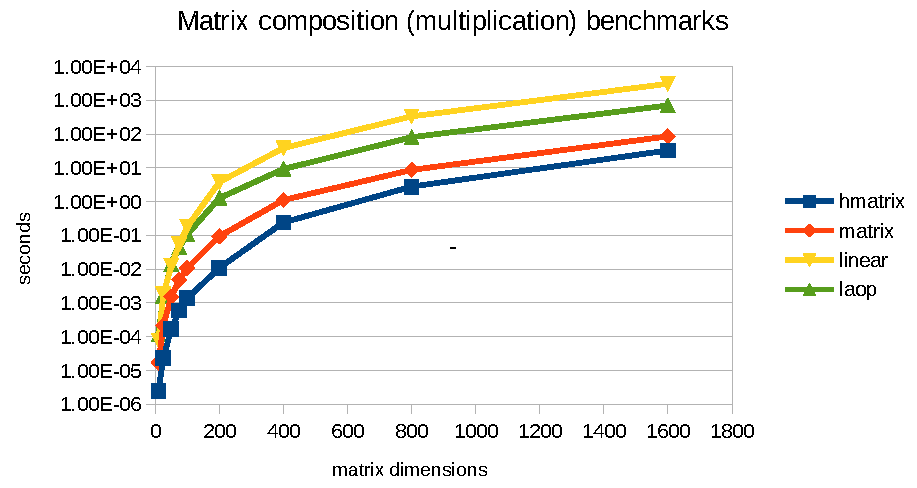
\includegraphics[width=\linewidth]{images/report1.pdf}
    \caption{Matrix composition benchmarks}
    \label{fig:bench}
\end{figure}

As can be seen in Figure \ref{fig:bench}, the \emph{hmatrix} and \emph{matrix} libraries are those that perform better. By observing their internal structure, one realises that they are a suitable representation for BLAS/LAPACK computations \cite{anderson1999lapack}, that is, they have been designed to efficiently exploit caches on modern cache-based architectures. A matrix in the \emph{linear} library is defined as \hs{Vector cols (Vector rows Double)} and does not take into account cache lengths or sizes, so it behaves much worse than the previous ones. Our structure does not take into account any low-level optimisations either, being unable to compete with those that do. Nevertheless, the implementation is \emph{performant for a cache-oblivious approach} and behaves better (almost one order of magnitude better) than other types of simpler definitions.

%Figure \ref{fig:bench2} plots a different set of benchmarks in which, instead of focusing on matrix multiplication alone, the more concrete and realistic case study provided by the query of \S\ref{subsec-data-analytics} was used as performance test.
% As we know, linear algebra's queen operation is the multiplication of matrices, and this is supposed to be the operation that has the greatest attention to optimisation. With this in mind and in order to compare the performance of different libraries in more concrete and realistic case studies, the results of the problem presented in \S\ref{subsec-data-analytics} 

%\begin{figure*}
%    \centering
%    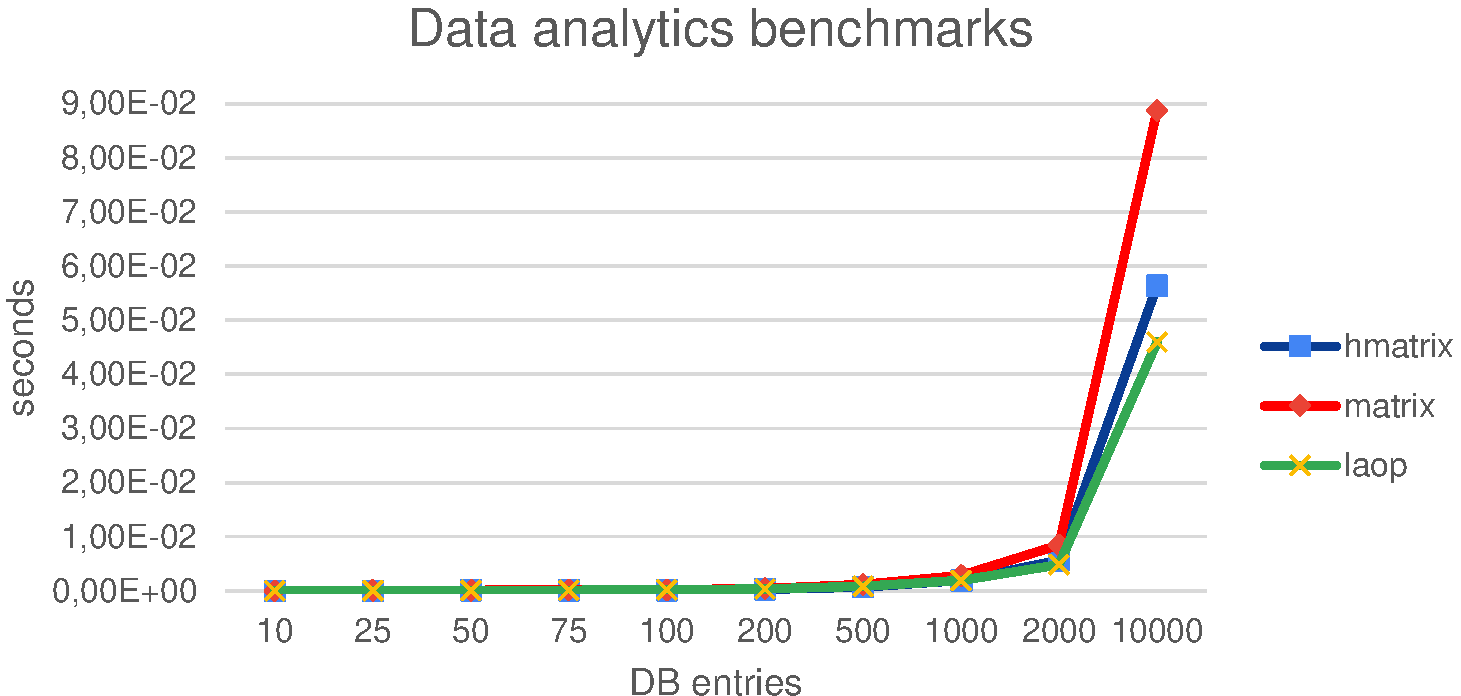
\includegraphics[width=0.495\textwidth]{images/report3.pdf}
%    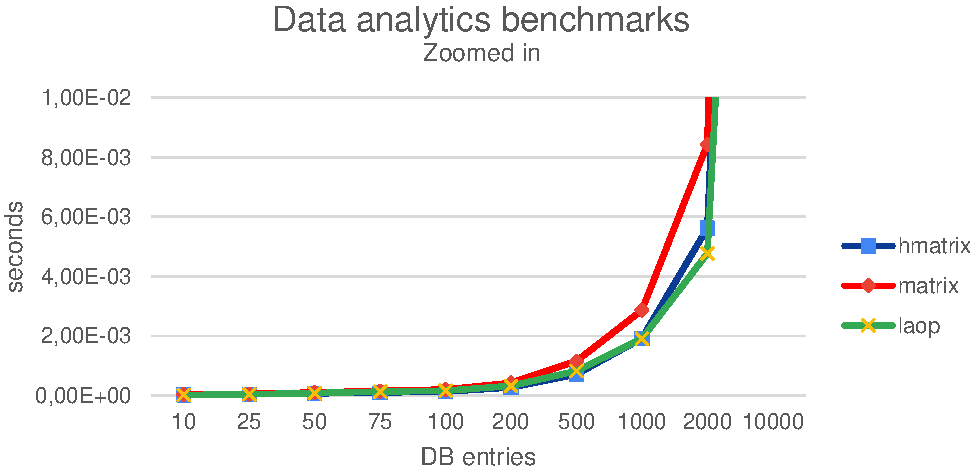
\includegraphics[width=0.495\textwidth]{images/report4.pdf}
%    \caption{Data analysis benchmark}
%    \label{fig:bench2}
%\end{figure*}
%
%In these benchmarks we only compared the performance of our library with those that provide much faster encoding with respect to matrix multiplication. As can be seen, there is no longer such a difference among libraries in this case study. This is due to the fact that, in the case of a real program, there are other operations with a greater impact than matrix composition. The results presented in Figure \ref{fig:bench2} show that our library is faster compared to the others. It should be noted that some of the operations (e.g. Khatri-Rao product) carried out in the competing libraries have been implemented with the help of conversions that incur a certain run-time overhead however, the price to be paid in relation to the performance/correction of the code is not that much.

%Still with regard to the example in \S\ref{subsec-data-analytics} the benefits go beyond code efficiency and scalability. The advantages of using a library which provides polymorphic and statically typed matrix manipulators \emph{\`a la} LAoP led to a painless implementation of a robust encoding of the query. More importantly, a method for inserting a new entry in the benchmark database was implemented in all evaluated libraries, and this was much simpler to do in rival libraries because it was done first and statically checked by ours.
%% Otherwise it would have been a solution that would have typed-checked and compiled, but far from having the same degree of trust.
%Concerning the query used in the benchmarks, it was much simpler to express it using our library and its typed combinators, not to mention that its implementation was much more straightforward and polymorphic than in the other competing libraries. 

%Section \ref{l-m-s} discussed a type-safer way of building elementary matrices, via linear map semantics, such as the projections used to implement the Khatri-Rao product, for example. Tests have been made for such alternatives, which unfortunately performed badly. (We intend to better understand why in future work.) So the benchmarks reported above did not use such safer but slower alternative implementations.

%\section{Functor and Arrow instances}
%
%Given the characterisation of \textbf{Mat}, where objects are the numerical dimensions and morphisms are matrices themselves, and since the \hs{Matrix} type provides explicit information about their dimensions, a valid instance of the \hs{Arrow} class should be possible to implement. However, as we already said, given that it is necessary to constrain the dimension types it is not possible to implement the \hs{Arrow} instance operators. The same happens when trying to implement \hs{Functor}, \hs{Selective} \cite{andrey2019selective}, \hs{Applicative} and \hs{Monad} instances. Nevertheless, it is possible to implement equivalent definitions, as is the case of the \hs{Applicative} instance where the \hs{Monoidal} correspondence translates to the Khatri-Rao matrix product.

\section{Related Work}\label{sec-related-work}

\emph{Algebraic graphs}~\cite{10.1145/3122955.3122956} were developed as an alternative to 
traditional graph representations, such as adjacency lists, with a focus on making it
impossible to describe ``malformed graphs'' where an edge refers to a non-existing vertex.
Algebraic graphs come with the following inductive definition:

\vspace{1mm}
\begin{minted}[xleftmargin=10pt]{haskell}
data Graph a where
    Empty   :: Graph a
    Vertex  :: a -> Graph a
    Overlay :: Graph a -> Graph a -> Graph a
    Connect :: Graph a -> Graph a -> Graph a
\end{minted}
\vspace{1mm}

\noindent
This data type is remarkably similar to our data type \hs{Matrix}: both have the ``singleton'' primitives, as well as a pair of binary operations. The resulting algebraic structures, however, are very different; instead of relations, algebraic graphs correspond to \emph{endo-relations}, i.e. relations whose domain and codomain coincide. As such, algebraic graphs are not directly applicable to our purposes. Interestingly, in the other direction one can use \hs{Matrix}~\hs{e}~\hs{c}~\hs{r} for representing \emph{weighted bipartite graphs}, i.e.\ graphs whose vertices are split into two parts~\hs{c} and~\hs{r} and edges have weights~\hs{e}.

Speaking of graphs and their relation to matrices, it is worth mentioning a functional pearl by~\citet{dolan2013fun} that describes how classic techniques from linear algebra can be used to solve a variety of graph (and non-graph) problems by formulating them as problems on \emph{matrices over semirings}. The paper mostly focuses on semirings and the reuse of ideas across multiple problem domains, making use of a very simple matrix representation:
\begin{minted}[xleftmargin=10pt]{haskell}
data Matrix a = Scalar a | Matrix [[a]]
\end{minted}
\noindent
What is particularly relevant to our work is that the algorithms used in the paper rely on
the decomposition of matrices into so-called ``block matrices'':
\begin{minted}[xleftmargin=10pt]{haskell}
type BlockMatrix a = (Matrix a, Matrix a,
                      Matrix a, Matrix a)
                      
msplit :: Matrix a -> BlockMatrix a
\end{minted}
\noindent
Since matrix dimensions are untyped, the implementation of \hs{msplit} and other matrix-manipulating functions described in the paper requires a great deal of care. By switching to our matrix representation, one can benefit from static correctness guarantees,  as well as exploit the inductive matrix definition whenever it needs to be decomposed into blocks.

As far as typed matrices are concerned, \citet{augustsson2016experience} and \citet{shaikhha2019finally} suggest approaches with similar objectives to ours. The results presented are in the form of a relational algebra library around a C++ library and a Scala matrix DSL that is polymorphic only in the content of the matrix. Relations can be seen as matrices and thus can be represented in our library as well, with all the advantages that are to be expected from using the inductive structure. The DSL approach allows one to provide several definitions of the
semiring/ring operation relative to the contents of the matrices, but they do not manipulate the matrices inductively, nor are their matrices dimensions polymorphic and statically typed.

\citet{El18} presents a vocabulary of matrices that introduces a minimal set of rules to build ``arbitrary matrices". This vocabulary is consistent with our inductive matrix structure. According to \cite{El18}, the vocabulary needed from generalised linear maps is exactly that of classes \hs{Category}, \hs{Cartesian}, \hs{Cocartesian} and \hs{Scalable}.
%(which he presents in his \doc)
Our API could evolve in this direction too. %complacent with this vocabulary, in its own restricted way, as we demonstrate in \S\ref{sec:cat}. So, it might be easy to apply such ideas in a more straightforward way.

\section{Conclusions and Future Work}\label{sec-conclusion}

%\begin{wrapfigure}[8]{r}{12em}
%~ 
%\begin{minipage}{11em}\footnotesize\em\vskip -1em
%``Using matrix notation such a set of simultaneous equations takes the form
%$A\comp x=b$ (...). In this way a set of equations has been reduced to a single equation. This is a tremendous improvement in concision that does not incur any loss
%of precision!''
%\vskip 1.0ex \em \hfill 
%Roland \citet{Ba04a}
%\end{minipage}
%\end{wrapfigure}

This paper proposes an inductive, block-oriented matrix definition that can be elegantly manipulated thanks to the algebraic laws of typed linear algebra. A solid, polymorphic, type-safe abstract API is provided that, thanks to the underlying theory, shows that one can create robust and efficient programs that rely on complex matrix manipulations. The examples show how well typed linear algebra blends with the functional programming style, providing an overall type-safe framework for the increased need in linear algebra based applications of our days, in areas such as data analysis and machine learning.

The proposed typed inductive matrix definition leads to efficient, cache-oblivious algorithms, such as matrix composition and transposition, allowing one to reason about code and write it in an elegant, type correct way.

We conclude that, although our encoding does not turn out to be better in terms of performance compared to more efficient libraries, it does not fall short of expectations and the expressiveness and simplicity that it offers justify its adoption. We understand our benchmarks are somewhat thin and plan to refine them in the future.

In future work we plan to fine-tune the implementation in several directions.
The block-oriented matrix type brings to mind quadtrees \cite{samet1984quadtree} and their savings wrt.\ repetitive cells (pixels). For sparse matrices, which have large blocks of zeros, an improved matrix definition catering for sparsity could be more efficient. Inspired by some of the limitations of the proposed inductive structure, such as the inability to have an unrestricted instance of \hs{Category} and to express large repetitive blocks, alternative formulations are to be explored. 

A possible approach could be based on making the type constructors more polymorphic.
%, at the cost of increasing the data type's complexity.
A new \hs{Identity} constructor could be added and \hs{One} could represent constant blocks of arbitrary sizes, by changing the unit type for polymorphic ones. Since the identity matrix should no longer possess associated dimension type restrictions, it should be possible to implement an unconstrained \hs{Category} instance offering a more efficient composition operation.
While we prefer our approach for its simplicity, a more complex inductive type promises advantages in type-safeness and space/time complexity.

Further to researching on a possibly extended encoding, studying how to take advantage of a fully type safe representation via linear map semantics or parallelization strategies to improve performance is also an interesting future direction.

%% Acknowledgements
\begin{acks} %% acks environment is optional
  %% contents suppressed with 'anonymous'
  %% Commands \grantsponsor{<sponsorID>}{<name>}{<url>} and
  %% \grantnum[<url>]{<sponsorID>}{<number>} should be used to
  %% acknowledge financial support and will be used by metadata
  %% extraction tools.

The authors wish to thank the anonymous referees for their comments and suggestions. They are also indebted to Andrey Mokhov for his constructive criticisms and, in particular, for many conversations on different possible interpretations of matrices and their relationships with algebraic graphs and Dolan's matrix representation.
% This work would likely have remained unpublished without his help and refinement.
Cláudia Correia, João Pereira and Eduardo Barbosa also provided constructive feedback on this paper, helping to substantially improve it. %Last but not least, we want to thank the whole Functional Programming community for having answered a number of code-related questions when developing my library.

While doing this work Armando Santos held a Research Grant of the DaVinci Project funded by FEDER (through the Operational Programme for Competitiveness and Internationalisation - COMPETE 2020 Programme) and by National Funds through the
    \grantsponsor{
            GS100000001
        }{
            FCT (Portuguese Foundation for Science and Technology, I.P.)
        }{
            http://dx.doi.org/10.13039/501100001871
        }
under Grant No.~\grantnum{GS100000001}{PTDC/CCI-COM/29946/2017}.

Any opinions, findings, and conclusions or recommendations expressed in this material are those of the authors and do not necessarily reflect the views of the funding agencies.
\end{acks}

%% Bibliography
\bibliography{bibfile}

%%% Appendix
%\appendix\small
%
%\section{Spreadsheets.hs}\label{appendix-spreadsheet}
%\begin{minted}[xleftmargin=10pt, mathescape=true]{haskell}
%{-# LANGUAGE DeriveGeneric #-}
%module Spreadsheets where
%
%import LAoP.Utils
%import LAoP.Matrix.Type
%import GHC.Generics
%import Prelude hiding (id, (.))
%
%data Student = Student1 | Student2 | Student3 | Student4
%  deriving (Eq, Show, Enum, Bounded, Generic)
%
%data Question = Question1 | Question2 | Question3 | Question4
%  deriving (Eq, Show, Enum, Bounded, Generic)
%
%data Results = Exam | Test | Final
%  deriving (Eq, Show, Enum, Bounded, Generic)
%
%test :: Matrix Float One Results
%test = point Test
%
%exam :: Matrix Float One Results
%exam = point Exam
%
%final :: Matrix Float One Results
%final = point Final
%
%w :: Matrix Float Question One
%w = matrixBuilder gen
%  where
%    gen (Question1, ()) = 0.2
%    gen (Question2, ()) = 0.3
%    gen (Question3, ()) = 0.2
%    gen (Question4, ()) = 0.3
%
%xls :: Matrix Float Question One
%    -> Matrix Float Question Student
%    -> Matrix Float Student One
%    -> Matrix Float (Either Question Results) (Either One Student)
%xls w m t = join (fork w m) (fork zeros r)
%  where
%    rExam = m . tr w
%    rTest = tr t
%    rFinal = rTest `maxPW` rExam
%    r = (rExam . tr exam) + (rTest . tr test) + (rFinal . tr final)
%
%-- | Overloaded, entry-wise 'max' function
%maxPW :: Ord e => Matrix e a b -> Matrix e a b -> Matrix e a b
%maxPW = zipWithM max
%\end{minted}
%
%\section{Sprinkler.hs}\label{appendix-sprinkler}
%\begin{minted}[xleftmargin=10pt, mathescape=true]{haskell}
%{-# LANGUAGE DeriveGeneric #-}
%module Sprinkler where
%  
%import LAoP.Utils
%import LAoP.Matrix.Type
%import GHC.Generics
%import Prelude hiding (id, (.))
%  
%data G = Dry | Wet
%    deriving (Bounded, Enum, Eq, Show, Generic)
%
%data S = Off | On
%    deriving (Bounded, Enum, Eq, Show, Generic)
%
%data R = No | Yes
%    deriving (Bounded, Enum, Eq, Show, Generic)
%    
%type Prob = Double
%
%rain :: Matrix Prob () R
%rain = matrixBuilder gen
%  where
%    gen ((), No)  = 0.8
%    gen ((), Yes) = 0.2
%
%sprinkler :: Matrix Prob R S
%sprinkler = matrixBuilder gen
%  where
%    gen (No, Off)  = 0.6
%    gen (No, On)   = 0.99
%    gen (Yes, Off) = 0.4
%    gen (Yes, On)  = 0.01
%
%grass :: Matrix Prob (S, R) G
%grass = matrixBuilder gen
%  where
%    gen ((Off, No), Dry)  = 1
%    gen ((Off, Yes), Dry) = 0.2
%    gen ((On, No), Dry)   = 0.1
%    gen ((On, Yes), Dry)  = 0.01
%    gen ((Off, No), Wet)  = 0
%    gen ((Off, Yes), Wet) = 0.8
%    gen ((On, No), Wet)   = 0.9
%    gen ((On, Yes), Wet)  = 0.99
%
%tag f = kr f id
%
%compose g s r = tag g . tag s . r
%
%grass_wet :: Matrix Prob () (G, (S, R)) -> Matrix Prob () ()
%grass_wet = tr (point Wet) . fstM
%
%main :: IO ()
%main = do
%    putStrLn "Probability of grass being wet:"
%    prettyPrint (grass_wet (compose grass sprinkler rain))
%\end{minted}

\end{document}
